\documentclass[14pt]{extarticle}

\usepackage{amsmath,mathtools,amsfonts,amsthm,amssymb,hyperref,cancel,tcolorbox}
\usepackage{wasysym,geometry,latexsym,parskip,bookmark,mathtools,float,xcolor}

\newtheorem{defn}{Definition}
\newtheorem{thm}{Theorem}
\newtheorem{claim}{Claim}
\newtheorem{lemma}{Lemma}

\newcommand{\dps}{\displaystyle}
\newcommand{\fbl}{\underline{\hspace{1cm}}\,\,}
\newcommand{\R}{\mathbb{R}}
\newcommand{\Z}{\mathbb{Z}}
\newcommand{\from}{\leftarrow}
\newcommand{\true}{{\bf t}}
\newcommand{\false}{{\bf c}}
\newcommand{\bic}{\leftrightarrow}

\hypersetup{colorlinks, allcolors=blue, linktoc=all}
\geometry{a4paper}
\geometry{margin=1.1cm}

\title{Chapter 2 Solutions, Susanna Epp Discrete Math 5th Edition}

\author{https://github.com/spamegg1}

\begin{document}
\maketitle
\tableofcontents

\section {Exercise Set 2.1}
{\bf In each of $1-4$ represent the common form of each argument using letters
to stand for component sentences, and fill in the blanks so that the argument in
part (b) has the same logical form as the argument in part (a).}

\subsection{Exercise 1}
\subsubsection{(a)}
If all integers are rational, then the number 1 is rational.

All integers are rational.

Therefore, the number 1 is rational.

\begin{proof}
Common form: 1) If $p$ then $q$. 2) $p$. 3) Therefore, $q$.
\end{proof}

\subsubsection{(b)}
If all algebraic expressions can be written in prefix notation, then \fbl.

Therefore, $(a + 2b)(a^2 - b)$ can be written in prefix notation.

\begin{proof}
If all algebraic expressions can be written in prefix notation, then \\
\underline{$(a + 2b)(a^2 - b)$ can be written in prefix notation.} (If $p$, then
$q$.)

All algebraic expressions can be written in prefix notation. ($p$.)

Therefore, $(a + 2b)(a^2 - b)$ can be written in prefix notation. (Therefore,
$q$.)
\end{proof}

\subsection{Exercise 2}
\subsubsection{(a)}
If all computer programs contain errors, then this program contains an error.

This program does not contain an error.

Therefore, it is not the case that all computer programs contain errors.

\begin{proof}
Common form: 1) If $p$ then $q$. 2) $\sim q$. 3) Therefore, $\sim p$.
\end{proof}

\subsubsection{(b)}
If \fbl then \fbl.

$2$ is not odd.

Therefore, it is not the case that all prime numbers are odd.

\begin{proof}
If \underline{all prime numbers are odd} then \underline{2 is odd}. (If $p$ then
$q$.)

$2$ is not odd. ($\sim q$.)

Therefore, it is not the case that all prime numbers are odd.
(Therefore, $\sim p$.)
\end{proof}

\subsection{Exercise 3}
\subsubsection{(a)}
This number is even or this number is odd.

This number is not even.

Therefore, this number is odd.

\begin{proof}
Common form: 1) $p \vee q$. 2) $\sim p$. 3) Therefore, $q$.
\end{proof}

\subsubsection{(b)}
\fbl or logic is confusing.

My mind is not shot.

Therefore, \fbl.

\begin{proof}
\underline{My mind is shot} or logic is confusing. ($p \vee q$.)

My mind is not shot. ($\sim p$.)

Therefore, \underline{logic is confusing}. (Therefore, $q$.)
\end{proof}

\subsection{Exercise 4}
\subsubsection{(a)}
If the program syntax is faulty, then the computer will generate an error
message.

If the computer generates an error message, then the program will not run.

Therefore, if the program syntax is faulty, then the program will not run.

\begin{proof}
Common form: 1) If $p$ then $q$. 2) If $q$ then $r$. 3) Therefore, if $p$ then
$r$.
\end{proof}

\subsubsection{(b)}
If this simple graph \fbl, then it is complete.

If this graph \fbl, then any two of its vertices can be joined by a path.

Therefore, if this simple graph has 4 vertices and 6 edges, then \fbl.

\begin{proof}
If this simple graph \underline{has 4 vertices and 6 edges}, then it is
complete.

If this graph \underline{is complete}, then any two of its vertices can be
joined by a path.

Therefore, if this simple graph has 4 vertices and 6 edges, then
\underline{any two of its vertices} \underline{can be joined by a path}.
\end{proof}

\subsection{Exercise 5}
Indicate which of the following sentences are statements.

\subsubsection{(a)}
1,024 is the smallest four-digit number that is a perfect square.

\begin{proof}
It is a statement because it is a true sentence. 1,024 is a perfect square
because $1,024 = 32^2$, and the next smaller perfect square is $31^2 = 961$,
which has fewer than four digits.
\end{proof}

\subsubsection{(b)}
She is a mathematics major.

\begin{proof}
It is not a statement because its truth value depends on the ``She''. (Here
``She'' can be thought of as a variable, like $x$.)
\end{proof}

\subsubsection{(c)}
$128 = 2^6$

\begin{proof}
It is a statement because it is false: $2^6 = 64 \neq 128$.
\end{proof}

\subsubsection{(d)}
$x = 2^6$

\begin{proof}
Not a statement, because its truth depends on the value of $x$.
\end{proof}

{\bf Write the statements in $6-9$ in symbolic form using the symbols $\sim$,
$\vee$ and $\wedge$ and the indicated letters to represent component
statements.}

\subsection{Exercise 6}
Let $s =$ “stocks are increasing” and $i =$ “interest rates are steady.”

\subsubsection{(a)}
Stocks are increasing but interest rates are steady.

\begin{proof}
$s \wedge i$.

(Notice that the ``but'' makes it sound like there should be a
negation involved, but that's just a quirk of English. In this case, ``but'' has
the same meaning as ``and''.

We have an intuitive expectation that there should be some ``causal link''
between stocks and interest rates, like: ``stocks are increasing, that should
affect interest rates'', so if the interest rates are remaining steady, it's as
if they are remaining steady DESPITE the fact that stocks are increasing, hence
the ``but'' being used.)
\end{proof}

\subsubsection{(b)}
Neither are stocks increasing nor are interest rates steady.

\begin{proof}
${\sim s} \wedge {\sim i}$.

(Another quirk of English: when ``neither nor'' is used, even though ``nor''
sounds like there should be an OR involved, it's actually AND and negation.)
\end{proof}

\subsection{Exercise 7}
Juan is a math major but not a computer science major. ($m =$ “Juan is a math
major,” $c =$ “Juan is a computer science major”)

\begin{proof}
$m \wedge {\sim c}$
\end{proof}

\subsection{Exercise 8}
Let $h =$ “John is healthy,” $w =$ “John is wealthy,” and
$s =$ “John is wise.”

\subsubsection{(a)}
John is healthy and wealthy but not wise.

\begin{proof}
$h \wedge w \wedge {\sim s}$.
\end{proof}

\subsubsection{(b)}
John is not wealthy but he is healthy and wise.

\begin{proof}
${\sim w} \wedge h \wedge s$.
\end{proof}

\subsubsection{(c)}
John is neither healthy, wealthy, nor wise.

\begin{proof}
${\sim h} \wedge {\sim w} \wedge {\sim s}$.
\end{proof}

\subsubsection{(d)}
John is neither wealthy nor wise, but he is healthy.

\begin{proof}
$({\sim w} \wedge {\sim s}) \wedge h$.
\end{proof}

\subsubsection{(e)}
John is wealthy, but he is not both healthy and wise.

\begin{proof}
$w \wedge {\sim (h \wedge s)}$.
\end{proof}

\subsection{Exercise 9}
Let $p =$ “$x > 5$,” $q =$ “$x = 5$,” and $r =$ “$10 > x$.”

\subsubsection{(a)}
$x \geq 5$

\begin{proof}
$x \geq 5$ means $x > 5$ or $x = 5$. So: $p \vee q$.
\end{proof}

\subsubsection{(b)}
$10 > x > 5$

\begin{proof}
$10 > x > 5$ means $10 > x$ and $x > 5$. So: $r \wedge p$.
\end{proof}

\subsubsection{(c)}
$10 > x \geq 5$

\begin{proof}
$10 > x \geq 5$ means $10 > x$ and $x \geq 5$, i.e. $10 > x$ and
($x > 5$ or $x = 5$).

So: $r \wedge (p \vee q)$.
\end{proof}

\subsection{Exercise 10}
Let $p$ be the statement “DATAENDFLAG is off,” $q$ the statement “ERROR equals
0,” and $r$ the statement “SUM is less than 1,000.” Express the following
sentences in symbolic notation.

\subsubsection{(a)}
DATAENDFLAG is off, ERROR equals 0, and SUM is less than 1,000.

\begin{proof}
$p \wedge q \wedge r$.
\end{proof}

\subsubsection{(b)}
DATAENDFLAG is off but ERROR is not equal to 0.

\begin{proof}
$p \wedge {\sim q}$.
\end{proof}

\subsubsection{(c)}
DATAENDFLAG is off; however, ERROR is not 0 or SUM is greater than or equal to
1,000.

\begin{proof}
$p \wedge ({\sim q} \vee {\sim r})$.
\end{proof}

\subsubsection{(d)}
DATAENDFLAG is on and ERROR equals 0 but SUM is greater than or equal to 1,000.

\begin{proof}
${\sim p} \wedge q \wedge {\sim r}$.
\end{proof}

\subsubsection{(e)}
Either DATAENDFLAG is on or it is the case that both ERROR equals 0 and SUM is
less than 1,000.

\begin{proof}
${\sim p} \vee (q \wedge r)$.
\end{proof}

\subsection{Exercise 11}
In the following sentence, is the word ``or'' used in its inclusive or exclusive
sense? A team wins the playoffs if it wins two games in a row or a total of
three games.

\begin{proof}
Inclusive or. For instance, a team could win the playoff by winning games 1, 3,
and 4 and losing game 2. Such an outcome would satisfy both conditions.
\end{proof}

{\bf Write truth tables for the statement forms in $12-15$.}

\subsection{Exercise 12}
${\sim p} \wedge q$

\begin{proof}
$$
\begin{array}{|cc|c|c|}
\hline
p & q & {\sim p} & {\sim p} \wedge q \\
\hline
T & T & F & F \\
\hline
T & F & F & F \\
\hline
F & T & T & T \\
\hline
F & F & T & F \\
\hline
\end{array}
$$
\end{proof}

\subsection{Exercise 13}
${\sim(p \wedge q)} \vee (p \vee q)$

\begin{proof}
This is a tautology:
$$
\begin{array}{|cc|c|c|c|c|c|}
\hline
p & q & p \wedge q & {\sim (p \wedge q)} & p \vee q & {\sim(p \wedge q)} \vee
(p \vee q) \\
\hline
T & T & T & F & T & T \\
\hline
T & F & F & T & T & T \\
\hline
F & T & F & T & T & T \\
\hline
F & F & F & T & F & T \\
\hline
\end{array}
$$
\end{proof}

\subsection{Exercise 14}
$p \wedge (q \wedge r)$

\begin{proof}
$$
\begin{array}{|ccc|c|}
\hline
p & q & r & p \wedge q \wedge r \\
\hline
T & T & T & T \\
\hline
T & T & F & F \\
\hline
T & F & T & F \\
\hline
T & F & F & F \\
\hline
F & T & T & F \\
\hline
F & T & F & F \\
\hline
F & F & T & F \\
\hline
F & F & F & F \\
\hline
\end{array}
$$
\end{proof}

\subsection{Exercise 15}
$p \wedge ({\sim q} \vee r)$

\begin{proof}
$$
\begin{array}{|ccc|c|c|}
\hline
p & q & r & {\sim q} \vee r & p \wedge ({\sim q} \vee r) \\
\hline
T & T & T & T & T \\
\hline
T & T & F & F & F \\
\hline
T & F & T & T & T \\
\hline
T & F & F & T & T \\
\hline
F & T & T & T & F \\
\hline
F & T & F & F & F \\
\hline
F & F & T & T & F \\
\hline
F & F & F & T & F \\
\hline
\end{array}
$$
\end{proof}

{\bf Determine whether the statement forms in $16-24$ are logically equivalent.
In each case, construct a truth table and include a sentence justifying your
answer. Your sentence should show that you understand the meaning of logical
equivalence.}

\subsection{Exercise 16}
$p \vee (p \wedge q)$ and $p$

\begin{proof}
$$
\begin{array}{|cc|c|c|}
\hline
p & q & p \wedge q & p \vee (p \wedge q) \\
\hline
T & T & T & T \\
\hline
T & F & F & T \\
\hline
F & T & F & F \\
\hline
F & F & F & F \\
\hline
\end{array}
$$

$p \vee (p \wedge q)$ and $p$ always have the same truth values, so they are
logically equivalent. (This proves one of the absorption laws.)
\end{proof}

\subsection{Exercise 17}
${\sim(p \wedge q)}$ and ${\sim p} \wedge {\sim q}$

\begin{proof}
$$
\begin{array}{|cc|c|c|}
\hline
p & q & {\sim(p \wedge q)} & {\sim p} \wedge {\sim q} \\
\hline
T & T & F & F \\
\hline
T & F & T & F \\
\hline
F & T & T & F \\
\hline
F & F & T & T \\
\hline
\end{array}
$$
Not logically equivalent. When $p = T$ and $q = F$ we have

${\sim (p \wedge q)} \equiv {\sim (T \wedge F)} \equiv {\sim F} \equiv T$, but

${\sim p} \wedge {\sim q} \equiv {\sim T \wedge {\sim F}} \equiv
F \wedge T \equiv F$.
\end{proof}

\subsection{Exercise 18}
$p \vee \true$ and \true

\begin{proof}
$$
\begin{array}{|cc|c|}
\hline
p & \true & p \vee \true \\
\hline
T & T & T \\
\hline
F & T & T \\
\hline
\end{array}
$$

$\true$ and $p \vee \true$ always have the same truth values, so they are
logically equivalent. (This proves one of the universal bound laws.)

\end{proof}

\subsection{Exercise 19}
$p \wedge \true$ and $p$

\begin{proof}
$$
\begin{array}{|cc|c|}
\hline
p & \true & p \wedge \true \\
\hline
T & T & T \\
\hline
F & T & F \\
\hline
\end{array}
$$

$p \wedge \true$ and $p$ always have the same truth values, so they are
logically equivalent.
\end{proof}

\subsection{Exercise 20}
$p \wedge \false$ and $p \vee \false$

\begin{proof}
$$
\begin{array}{|cc|c|c|}
\hline
p & \false & p \wedge \false & p \vee \false \\
\hline
T & F & F & T \\
\hline
F & F & F & F \\
\hline
\end{array}
$$

$p \wedge \false$ and $p \vee \false$ are not logically equivalent.
\end{proof}

\subsection{Exercise 21}
$(p \wedge q) \wedge r$ and $p \wedge (q \wedge r)$

\begin{proof}
$$
\begin{array}{|ccc|c|c|c|c|}
\hline
p & q & r & p \wedge q & q \wedge r & (p \wedge q) \wedge r &
p \wedge (q \wedge r) \\
\hline
T & T & T & T & T & T & T \\
\hline
T & T & F & T & F & F & F \\
\hline
T & F & T & F & F & F & F \\
\hline
T & F & F & F & F & F & F \\
\hline
F & T & T & F & T & F & F \\
\hline
F & T & F & F & F & F & F \\
\hline
F & F & T & T & F & F & F \\
\hline
F & F & F & F & F & F & F \\
\hline
\end{array}
$$

$(p \wedge q) \wedge r$ and $p \wedge (q \wedge r)$ always have the same truth
values, so they are logically equivalent. (This proves the associative law for
$\wedge$.)
\end{proof}

\subsection{Exercise 22}
$p \wedge (q \vee r)$ and $(p \wedge q) \vee (p \wedge r)$

\begin{proof}
$$
\begin{array}{|ccc|c|c|c|c|c|}
\hline
p & q & r & p \wedge q & p \wedge r & q \vee r & p \wedge (q \vee r) &
(p \wedge q) \vee (p \wedge r) \\
\hline
T & T & T & T & T & T & T & T \\
\hline
T & T & F & T & F & T & T & T \\
\hline
T & F & T & F & T & T & T & T \\
\hline
T & F & F & F & F & F & F & F \\
\hline
F & T & T & F & F & T & F & F \\
\hline
F & T & F & F & F & T & F & F \\
\hline
F & F & T & F & F & T & F & F \\
\hline
F & F & F & F & F & F & F & F \\
\hline
\end{array}
$$

$p \wedge (q \vee r)$ and $(p \wedge q) \vee (p \wedge r)$ always have the same
truth values, so they are logically equivalent. (This proves one of the
distributive laws for $\wedge$.)
\end{proof}

\subsection{Exercise 23}
$(p \wedge q) \vee r$ and $p \wedge (q \vee r)$

\begin{proof}
$$
\begin{array}{|ccc|c|c|c|c|}
\hline
p & q & r & p \wedge q & q \vee r & (p \wedge q) \vee r & p \wedge (q \vee r)
\\\hline
T & T & T & T & T & T & T \\
\hline
T & T & F & T & T & T & T \\
\hline
T & F & T & F & T & T & T \\
\hline
T & F & F & F & F & F & F \\
\hline
F & T & T & F & T & T & F \\
\hline
F & T & F & F & T & F & F \\
\hline
F & F & T & F & T & T & F \\
\hline
F & F & F & F & F & F & F \\
\hline
\end{array}
$$

$(p \wedge q) \vee r$ and $p \wedge (q \vee r)$ have different truth values in
the fifth and seventh rows, so they are not logically equivalent. (This proves
that parentheses are needed with $\wedge$ and $\vee$.)
\end{proof}

\subsection{Exercise 24}
$(p \vee q) \vee (p \wedge r)$ and $(p \vee q) \wedge r$

\begin{proof}
$$
\begin{array}{|ccc|c|c|c|c|}
\hline
p & q & r & p \vee q & p \wedge r & (p \vee q) \vee (p \wedge r) &
(p \vee q) \wedge r \\
\hline
T & T & T & T & T & T & T \\
\hline
T & T & F & T & F & T & F \\
\hline
T & F & T & T & T & T & T \\
\hline
T & F & F & T & F & T & F \\
\hline
F & T & T & T & F & T & T \\
\hline
F & T & F & T & F & T & F \\
\hline
F & F & T & F & F & F & F \\
\hline
F & F & F & F & F & F & F \\
\hline
\end{array}
$$

$(p \vee q) \vee (p \wedge r)$ and $(p \vee q) \wedge r$ have different truth
values in the fifth and seventh rows, so they are not logically equivalent.
\end{proof}

{\bf Use De Morgan’s laws to write negations for the statements in $25-30$.}

\subsection{Exercise 25}
Hal is a math major and Hal’s sister is a computer science major.

\begin{proof}
$p =$ Hal is a math major, $q =$ Hal’s sister is a computer science major

The statement is $p \wedge q$. By De Morgan's laws, the negation is $\sim(p
\wedge q) \equiv {\sim p} \vee {\sim q}$:

Hal is not a math major, or Hal's sister is not a computer science major.
\end{proof}

\subsection{Exercise 26}
Sam is an orange belt and Kate is a red belt.

\begin{proof}
$p =$ Sam is an orange belt, $q =$ Kate is a red belt.

The statement is $p \wedge q$. By De Morgan's laws, the negation is $\sim(p
\wedge q) \equiv {\sim p} \vee {\sim q}$:

Sam is not an orange belt, or Kate is not a red belt.
\end{proof}

\subsection{Exercise 27}
The connector is loose or the machine is unplugged.

\begin{proof}
$p =$ The connector is loose, $q =$ the machine is unplugged.

The statement is $p \vee q$. By De Morgan's laws, the negation is $\sim(p \vee
q) \equiv {\sim p} \wedge {\sim q}$:

The connector is not loose and the machine is not unplugged.
\end{proof}

\subsection{Exercise 28}
The train is late or my watch is fast.

\begin{proof}
$p =$ The train is late, $q =$ my watch is fast.

The statement is $p \vee q$. By De Morgan's laws, the negation is $\sim(p \vee
q) \equiv {\sim p} \wedge {\sim q}$:

The train is not late and my watch is not fast.
\end{proof}

\subsection{Exercise 29}
This computer program has a logical error in the first ten lines or it is being
run with an incomplete data set.

\begin{proof}
$p =$ This computer program has a logical error in the first ten lines,

$q =$ it (this computer) is being run with an incomplete data set.

The statement is $p \vee q$. By De Morgan's laws, the negation is $\sim(p \vee
q) \equiv {\sim p} \wedge {\sim q}$:

This computer program does not have a logical error in the first ten lines and
it is not being run with an incomplete data set.
\end{proof}

\subsection{Exercise 30}
The dollar is at an all-time high and the stock market is at a record low.

\begin{proof}
$p =$ The dollar is at an all-time high, $q =$ the stock market is at a record
low.

The statement is $p \wedge q$. By De Morgan's laws, the negation is $\sim(p
\wedge q) \equiv {\sim p} \vee {\sim q}$:

The dollar is not at an all-time high or the stock market is not at a record
low.
\end{proof}

\subsection{Exercise 31}
Let $s$ be a string of length $2$ with characters from $\{0, 1, 2\}$, and define
statements $a, b, c$, and $d$ as follows:

\begin{itemize}
\item $a = $ ``the first character of $s$ is $0$''
\item $b = $ ``the first character of $s$ is $1$''
\item $c = $ ``the second character of $s$ is $1$''
\item $d = $ ``the second character of $s$ is $2$''
\end{itemize}

Describe the set of all strings for which each of the following is true.

(Here are all the possible length 2 strings: 00, 01, 02, 10, 11, 12, 20, 21, 22)
\subsubsection{(a)}
$(a \vee b) \wedge (c \vee d)$

\begin{proof}
This translates to: ``the first character is 0 or 1, and the second character
is1 or 2''. So the answer is: 01, 02, 11, 12
\end{proof}

\subsubsection{(b)}
$({\sim(a \vee b)}) \wedge (c \vee d)$

\begin{proof}
This translates to: ``the first character is not 0 or 1, and the second
character is 1 or 2''. So the answer is: 21, 22
\end{proof}

\subsubsection{(c)}
$(({\sim a}) \vee b) \wedge (c \vee ({\sim d}))$

\begin{proof}
This translates to: ``the first character is not 0 or it is 1, and the second
character is 1 or is not 2''.

So the first character can be 1 or 2, and the second character can be 0 or 1.

So the answer is: 10, 11, 20, 21
\end{proof}

{\bf Assume $x$ is a particular real number and use De Morgan’s laws to write
negations for the statements in $32-37$.}

\subsection{Exercise 32}
$-2 < x < 7$

\begin{proof}
This is $(-2 < x) \wedge (x < 7)$. Keep in mind that the negation of $<$ is
$\geq$. By De Morgan, the negation is

$\sim((-2 < x) \wedge (x < 7)) \equiv {\sim(-2 < x)} \vee {\sim(x < 7)} \equiv
(-2 \geq x) \vee (x \geq 7)$

The answer is: $-2 \geq x$ or $x \geq 7$.
\end{proof}

\subsection{Exercise 33}
$-10 < x < 2$

\begin{proof}
Similar to 32, the answer is: $-10 \geq x$ or $x \geq 2$.
\end{proof}

\subsection{Exercise 34}
$x < 2$ or $x > 5$

\begin{proof}
The negation of $>$ is $\leq$. By De Morgan, the negation is:

${\sim(x < 2 \vee x > 5)} \equiv {\sim (x < 2)} \wedge {\sim (x > 5)} \equiv (x
\geq 2) \wedge (x \leq 5)$

The answer is: $2 \leq x \leq 5$.
\end{proof}

\subsection{Exercise 35}
$x \leq -1$ or $x > 1$

\begin{proof}
Similar to 34. The answer is: $-1 < x \leq 1$.
\end{proof}

\subsection{Exercise 36}
$1 > x \geq -3$

\begin{proof}
Rewriting this as $-3 \leq x < 1$, we see that it is similar to 32 and 33.

The answer is: $-3 > x$ or $x \geq 1$. In other words: $1 \leq x$ or $x < -3$.
\end{proof}

\subsection{Exercise 37}
$0 > x \geq -7$

\begin{proof}
This is just like 36. The answer is: $0 \leq x$ or $x < -7$.
\end{proof}

{\bf In 38 and 39, imagine that {\it num\_orders} and {\it num\_instock} are
particular values, such as might occur during execution of a computer program.
Write negations for the following statements.}

\subsection{Exercise 38}
$(num\_orders > 100$ and $num\_instock \leq 500)$ or $num\_instock < 200$

\begin{proof}
This statement’s logical form is $(p \wedge q) \vee r$, so its negation has the
form

$$
{\sim((p \wedge q) \vee r)} \equiv {\sim (p \wedge q)} \wedge {\sim r}
\equiv ({\sim p} \vee {\sim q}) \wedge {\sim r}
$$

Thus a negation for the statement is:

$(num\_orders \leq 100$ or $num\_instock > 500)$ and $num\_instock \geq 200$.
\end{proof}

\subsection{Exercise 39}
$(num\_orders < 50$ and $num\_instock > 300)$ or

$(50 \leq num\_orders < 75$ and $num\_instock > 500)$

\begin{proof}
This statement’s logical form is $(p \wedge q) \vee ({\sim p} \wedge r \wedge
s)$, so its negation has the form

$$
{\sim((p \wedge q) \vee ({\sim p} \wedge r \wedge s))} \equiv
{\sim(p \wedge q)} \wedge {\sim({\sim p} \wedge r \wedge s)} \equiv
({\sim p} \vee {\sim q}) \wedge (p \vee {\sim r} \vee {\sim s})
$$

Thus a negation for the statement is:

$(num\_orders \geq 50$ or $num\_instock \leq 300)$ and

($num\_orders < 50$ or $num\_orders \geq 75$ or $num\_instock \leq 500$).
\end{proof}

{\bf Use truth tables to establish which of the statement forms in $40-43$ are
tautologies and which are contradictions.}

\subsection{Exercise 40}
$(p \wedge q) \vee ({\sim p} \vee (p \wedge {\sim q}))$

\begin{proof}
$$
\begin{array}{|cc|c|c|c|c|c|c|}
\hline
p & q & {\sim p} & {\sim q} & p \wedge q & p \wedge {\sim q} &
{\sim p} \vee (p \wedge {\sim q}) &
(p \wedge q) \vee ({\sim p} \vee (p \wedge {\sim q})) \\
\hline
T & T & F & F & T & F & F & T \\
\hline
T & F & F & T & F & T & T & T \\
\hline
F & T & T & F & F & F & T & T \\
\hline
F & F & T & T & F & F & T & T \\
\hline
\end{array}
$$
We see that $(p \wedge q) \vee ({\sim p} \vee (p \wedge {\sim q}))$ is a
tautology.
\end{proof}

\subsection{Exercise 41}
$(p \wedge {\sim q}) \wedge ({\sim p} \vee q))$

\begin{proof}
$$
\begin{array}{|cc|c|c|c|c|c|}
\hline
p & q & {\sim p} & {\sim q} & p \wedge {\sim q} & {\sim p} \vee q &
(p \wedge {\sim q}) \wedge ({\sim p} \vee q) \\
\hline
T & T & F & F & F & T & F  \\
\hline
T & F & F & T & T & F & F  \\
\hline
F & T & T & F & F & T & F  \\
\hline
F & F & T & T & F & T & F  \\
\hline
\end{array}
$$
\end{proof}
$(p \wedge {\sim q}) \wedge ({\sim p} \vee q)$ is always false, so it is a
contradiction.


\subsection{Exercise 42}
$(({\sim p} \wedge q) \wedge (q \wedge r))) \wedge {\sim q}$

\begin{proof}
$$
\begin{array}{|ccc|c|c|c|c|}
\hline
p & q & r & {\sim p} \vee q & q \wedge r & ({\sim p} \vee q) \wedge (q \wedge
r)& (({\sim p} \wedge q) \wedge (q \wedge r))) \wedge {\sim q} \\
\hline
T & T & T & T & T & T & F \\
\hline
T & T & F & T & F & F & F \\
\hline
T & F & T & F & F & F & F \\
\hline
T & F & F & F & F & F & F \\
\hline
F & T & T & T & T & T & F \\
\hline
F & T & F & T & F & F & F \\
\hline
F & F & T & T & F & F & F \\
\hline
F & F & F & T & F & F & F \\
\hline
\end{array}
$$
$(({\sim p} \wedge q) \wedge (q \wedge r))) \wedge {\sim q}$ is a contradiction.
\end{proof}

\subsection{Exercise 43}
$({\sim p} \vee q) \vee (p \wedge {\sim q})$

\begin{proof}
$$
\begin{array}{|cc|c|c|c|c|c|}
\hline
p & q & {\sim p} & {\sim q} & {\sim p} \vee q & p \wedge {\sim q} &
({\sim p} \vee q) \vee (p \wedge {\sim q}) \\
\hline
T & T & F & F & T & F & T \\
\hline
T & F & F & T & F & T & T \\
\hline
F & T & T & F & T & F & T \\
\hline
F & F & T & T & T & F & T \\
\hline
\end{array}
$$
We see that $({\sim p} \vee q) \vee (p \wedge {\sim q})$ is a tautology.
\end{proof}

\subsection{Exercise 44}
Recall that $a < x < b$ means that $a < x$ and $x < b$. Also $a \leq b$ means
that $a < b$ or $a = b$. Find all real numbers $x$ that satisfy the following
inequalities.

\subsubsection{(a)}
$2 < x \leq 0$

\begin{proof}
No real numbers satisfy this inequality. If $x > 2$ then $x > 2 > 0$ so $x >
0$.Therefore $x \leq 0$ cannot be true at the same time.
\end{proof}

\subsubsection{(b)}
$1 \leq x < -1$

\begin{proof}
Similar to (a). no real numbers satisfy this inequality.
\end{proof}

\subsection{Exercise 45}
Determine whether the statements in (a) and (b) are logically equivalent.

(a)
Bob is both a math and computer science major and Ann is a math major, but Ann
is not both a math and computer science major.

(b)
It is not the case that both Bob and Ann are both math and computer science
majors, but it is the case that Ann is a math major and Bob is both a math and
computer science major.

\begin{proof}
Define
\begin{enumerate}
\item $p$: Bob is a math major.
\item $q$: Bob is a CS major.
\item $r$: Ann is a math major.
\item $s$: Ann is a CS major.
\end{enumerate}

The statement in (a) has the form:
$(p \wedge q \wedge r) \wedge {\sim (r \wedge s)}$

The statement in (b) has the form:
${\sim (p \wedge q \wedge r \wedge s)} \wedge (r \wedge p \wedge q)$

We could write down the entire truth table with $2^4 = 16$ rows, but let's try
to take some shortcuts.

If we look at the two expressions, they both have the form
$(p \wedge q \wedge r) \wedge Z$. Such an expression is true when $(p \wedge q
\wedge r)$ and $Z$ are both true, and it is false otherwise.

Therefore, when evaluating $Z$, we can concentrate only on the rows of the truth
table where $(p \wedge q \wedge r)$ is true. We can disregard $Z$ on the other
rows (because both (a) and (b) are false for those rows).

$(p \wedge q \wedge r)$ is true only when all 3 of $p, q, r$ are true. When this
is the case, we only need to consider the possibilities for $s$. This gives us 2
rows only:
$$
\begin{array}{|c|c|c|}
\hline
s & {\sim (r \wedge s)} & {\sim (p \wedge q \wedge r \wedge s)} \\
\hline
T & F & F \\
\hline
F & T & T \\
\hline
\end{array}
$$

The two $Z$ expressions have the same truth values in all cases. Therefore (a)
and (b) are logically equivalent.
\end{proof}

\subsection{Exercise 46}
Let the symbol $\oplus$ denote {\it exclusive or}; so $p \oplus q \equiv (p \vee
q) \wedge {\sim(p \wedge q)}$. Hence the truth table for $p \oplus q$ is as
follows:

\begin{center}
\begin{tabular}{|cc|c|}
\hline
$p$ & $q$ & $p \oplus q$ \\
\hline
T & T & F \\
\hline
T & F & T \\
\hline
F & T & T \\
\hline
F & F & F \\
\hline
\end{tabular}
\end{center}

\subsubsection{(a)}
Find simpler statement forms that are logically equivalent to $p \oplus p$ and
$(p \oplus p) \oplus p$.

\begin{proof}
The meaning of the exclusive or $\oplus$ is that, it returns true when the two
operands have different truth values; otherwise it returns false.

In $p \oplus p$, the two operands $p$ and $p$ always have the same truth value.
Therefore $p \oplus p$ is a contradiction: $p \oplus p \equiv \false$.

So we have $(p \oplus p) \oplus p \equiv \false \oplus p$. This is true only
when $p$ and $\false$ have different truth values, in other words, when $p$ is
true. Therefore $\false \oplus p$ is logically equivalent to $p$.
\end{proof}

\subsubsection{(b)}
Is $(p \oplus q) \oplus r \equiv p \oplus (q \oplus r)$? Justify your answer.

\begin{proof}
$$
\begin{array}{|ccc|c|c|c|c|}
\hline
p & q & r & p \oplus q & q \oplus r & (p \oplus q) \oplus r & 
p \oplus (q \oplus r) \\
\hline
T & T & T & F & F & T & T \\
\hline
T & T & F & F & T & F & F \\
\hline
T & F & T & T & T & F & F \\
\hline
T & F & F & T & F & T & T \\
\hline
F & T & T & T & F & F & F \\
\hline
F & T & F & T & T & T & T \\
\hline
F & F & T & F & T & T & T \\
\hline
F & F & F & F & F & F & F \\
\hline
\end{array}
$$
They are logically equivalent.
\end{proof}

\subsubsection{(c)}
Is $(p \oplus q) \wedge r \equiv (p \wedge r) \oplus (q \wedge r)$? Justify your
answer.

\begin{proof}
$$
\begin{array}{|ccc|c|c|c|c|c|}
\hline
p & q & r & p \oplus q & p \wedge r & q \wedge r & 
(p \oplus q) \wedge r & (p \wedge r) \oplus (q \wedge r) \\
\hline
T & T & T & F & T & T & F & T \\
\hline
T & T & F & F & F & F & F & T \\
\hline
T & F & T & T & T & F & T & T \\
\hline
T & F & F & T & F & F & F & T \\
\hline
F & T & T & T & F & T & T & F \\
\hline
F & T & F & T & F & F & F & F \\
\hline
F & F & T & F & F & F & F & F \\
\hline
F & F & F & F & F & F & F & F \\
\hline
\end{array}
$$
They are NOT logically equivalent.
\end{proof}

\subsection{Exercise 47}
In logic and in standard English, a double negative is equivalent to a
positive.There is one fairly common English usage in which a “double positive”
is equivalent to a negative. What is it? Can you think of others?

\begin{proof}
There is a famous story about a philosopher who once gave a talk in which he
observed that whereas in English and many other languages a double negative is
equivalent to a positive, there is no language in which a double positive is
equivalent to a negative. To this, another philosopher, Sidney Morgenbesser,
responded sarcastically, “Yeah, yeah.”

{\it [Strictly speaking, sarcasm functions like negation. When spoken
sarcastically, the words “Yeah, yeah” are not a true double positive; they just
mean “no.”]}
\end{proof}

In 48 and 49 below, a logical equivalence is derived from Theorem 2.1.1. Supply
a reason for each step.

\subsection{Exercise 48}
$$
\begin{array}{rcll}
(p \wedge {\sim q}) \vee (p \wedge q) & \equiv & 
 p \wedge ({\sim q} \vee q) & \text{by (a)} \\
& \equiv & p \wedge (q \vee {\sim q}) & \text{by (b)} \\
& \equiv & p \wedge \true & \text{by (c)} \\
& \equiv & p & \text{by (d)} \\
\end{array}
$$

Therefore, $(p \wedge {\sim q}) \vee (p \wedge q) \equiv p$.

\begin{proof}
(a) is the distributive law. (b) is the commutative law for $\vee$. (c) is the
negation law for $\vee$. (d) is the identity law for $\wedge$.
\end{proof}

\subsection{Exercise 49}
$$
\begin{array}{rcll}
(p \vee {\sim q}) \wedge ({\sim p} \vee {\sim q}) & \equiv &
({\sim q} \vee p) \wedge ({\sim q} \vee {\sim p}) & \text{by (a)} \\
& \equiv & {\sim q} \vee (p \wedge {\sim p}) & \text{by (b)} \\
& \equiv & {\sim q} \vee \false & \text{by (c)} \\
& \equiv & {\sim q} & \text{by (d)} \\
\end{array}
$$

Therefore, $(p \vee {\sim q}) \wedge ({\sim p} \vee {\sim q}) \equiv {\sim q}$.

\begin{proof}
(a) is the commutative law for $\vee$. (b) is the distributive law. (c) is the
negation law for $\wedge$. (d) is the identity law for $\vee$.
\end{proof}

{\bf Use Theorem 2.1.1 to verify the logical equivalences in $50-54$. Supply a
reason for each step.}

\subsection{Exercise 50}
$(p \wedge {\sim q}) \vee p \equiv p$

\begin{proof}
$(p \wedge {\sim q}) \vee p$

\begin{tabular}{rclr}
& $\equiv$ & $p \vee (p \wedge {\sim q})$ & (by the commutative law for $\vee$)
\\
 & $\equiv$ & $p$ & (by the absorption law for $\vee$) \\
\end{tabular}
\end{proof}

\subsection{Exercise 51}
$p \wedge ({\sim q} \vee p) \equiv p$

\begin{proof}
$p \wedge ({\sim q} \vee p)$

\begin{tabular}{rclr}
& $\equiv$ & $p \wedge (p \vee {\sim q})$ & (by the commutative law for $\vee$)
\\
 & $\equiv$ & $p$ & (by the absorption law for $\wedge$) \\
\end{tabular}
\end{proof}

\subsection{Exercise 52}
${\sim (p \vee {\sim q})} \vee ({\sim p} \wedge {\sim q}) \equiv {\sim p}$

\begin{proof}
${\sim (p \vee {\sim q})} \vee ({\sim p} \wedge {\sim q})$ 

\begin{tabular}{rcll}
& $\equiv$ & $({\sim p} \wedge q) \vee ({\sim p} \wedge {\sim q})$ & (by De
Morgan laws) \\
& $\equiv$ & ${\sim p} \wedge (q \vee {\sim q})$ & (by distributive law for
$\wedge$) \\
 & $\equiv$ & ${\sim p} \wedge \true$ & (by negation law for $\vee$) \\
 & $\equiv$ & ${\sim p}$ & (by identity law for $\wedge$) \\
\end{tabular}
\end{proof}

\subsection{Exercise 53}
$\sim(({\sim p} \wedge q) \vee ({\sim p} \wedge {\sim q})) \vee (p \wedge q)
\equiv p$

\begin{proof}
$\sim(({\sim p} \wedge q) \vee ({\sim p} \wedge {\sim q})) \vee (p \wedge q)$

\begin{tabular}{rcll}
& $\equiv$ & $\sim({\sim p} \wedge (q \vee {\sim q})) \vee (p \wedge q)$ & (by
the distributive law) \\
 & $\equiv$ & $\sim({\sim p} \wedge \true) \vee (p \wedge q)$ &
(by the negation law for $\vee$) \\
& $\equiv$ & $\sim({\sim p}) \vee (p \wedge q)$ & (by the identity law for
$\vee$) \\
 & $\equiv$ & $p \vee (p \wedge q)$ & (by the double negative law) \\
 & $\equiv$ & $p$ & (by the absorption law) \\
\end{tabular}
\end{proof}

\subsection{Exercise 54}
$(p \wedge ({\sim ({\sim p} \vee q)})) \vee (p \wedge q) \equiv p$

\begin{proof}
$(p \wedge ({\sim ({\sim p} \vee q)})) \vee (p \wedge q)$

\begin{tabular}{rcll}
 & $\equiv$ & 
$(p \wedge (p \wedge {\sim q})) \vee (p \wedge q)$ & (by De Morgan law) \\
& $\equiv$ & $((p \wedge p) \wedge {\sim q}) \vee (p \wedge q)$ & (by the
associative law) \\
& $\equiv$ & $(p \wedge {\sim q}) \vee (p \wedge q)$ & (by the idempotent law)
\\
 & $\equiv$ & $p \wedge ({\sim q} \vee q)$ & (by the distributive law) \\
 & $\equiv$ & $p \wedge \true$ & (by the negation law) \\
 & $\equiv$ & $p$ & (by the identity law) \\
\end{tabular}
\end{proof}

\section{Exercise Set 2.2}
{\bf Rewrite the statements in $1-4$ in if-then form.}

\subsection{Exercise 1}
This loop will repeat exactly $N$ times if it does not contain a stop or a go
to.

\begin{proof}
If this loop does not contain a stop or a go to, then it will repeat exactly $N$
times.
\end{proof}

\subsection{Exercise 2}
I am on time for work if I catch the 8:05 bus.

\begin{proof}
If I catch the 8:05 bus then I am on time for work.
\end{proof}

\subsection{Exercise 3}
Freeze or I’ll shoot.

\begin{proof}
If you do not freeze, then I’ll shoot.
\end{proof}

\subsection{Exercise 4}
Fix my ceiling or I won’t pay my rent.

\begin{proof}
If you do not fix my ceiling then I won't pay my rent.
\end{proof}

{\bf Construct truth tables for the statement forms in $5-11$.}

\subsection{Exercise 5}
${\sim p} \vee q \to {\sim q}$

\begin{proof}
$$
\begin{array}{|cc|c|c|c|c|}
\hline
p & q & {\sim p} & {\sim q} & {\sim p} \vee q & {\sim p} \vee q \to {\sim q} \\
\hline
T & T & F & F & T & F \\
\hline
T & F & F & T & F & T \\
\hline
F & T & T & F & T & F \\
\hline
F & F & T & T & T & T \\
\hline
\end{array}
$$
\end{proof}

\subsection{Exercise 6}
$(p \vee q) \vee ({\sim p} \wedge q) \to q$

\begin{proof}
$$
\begin{array}{|cc|c|c|c|c|c|}
\hline
p & q & {\sim p} & p \vee q & {\sim p} \wedge q & (p \vee q) \vee ({\sim p}
\wedge q) & (p \vee q) \vee ({\sim p} \wedge q) \to q \\
\hline
T & T & F & T & F & T & T \\
\hline
T & F & F & T & F & T & F \\
\hline
F & T & T & T & T & T & T \\
\hline
F & F & T & F & F & F & T \\
\hline
\end{array}
$$
\end{proof}

\subsection{Exercise 7}
$p \wedge {\sim q} \to r$

\begin{proof}
$$
\begin{array}{|ccc|c|c|c|}
\hline
p & q & r & {\sim q} & p \wedge {\sim q} & p \wedge {\sim q} \to r \\
\hline
T & T & T & F & F & T \\
\hline
T & T & F & F & F & T \\
\hline
T & F & T & T & T & T \\
\hline
T & F & F & T & T & F \\
\hline
F & T & T & F & F & T \\
\hline
F & T & F & F & F & T \\
\hline
F & F & T & T & F & T \\
\hline
F & F & F & T & F & T \\
\hline
\end{array}
$$
\end{proof}

\subsection{Exercise 8}
${\sim p} \vee q \to r$

\begin{proof}
$$
\begin{array}{|ccc|c|c|c|}
\hline
p & q & r & {\sim p} & {\sim p} \vee q & {\sim p} \vee q \to r \\
\hline
T & T & T & F & T & T \\
\hline
T & T & F & F & T & F \\
\hline
T & F & T & F & F & T \\
\hline
T & F & F & F & F & T \\
\hline
F & T & T & T & T & T \\
\hline
F & T & F & T & T & F \\
\hline
F & F & T & T & T & T \\
\hline
F & F & F & T & T & F \\
\hline
\end{array}
$$
\end{proof}

\subsection{Exercise 9}
$p \wedge {\sim r} \bic q \vee r$

\begin{proof}
$$
\begin{array}{|ccc|c|c|c|c|}
\hline
p & q & r & {\sim r} & p \wedge {\sim r} & q \vee r & p \wedge {\sim r} \bic q
\vee r \\
\hline
T & T & T & F & F & T & F \\
\hline
T & T & F & T & T & T & T \\
\hline
T & F & T & F & F & T & F \\
\hline
T & F & F & T & T & F & F \\
\hline
F & T & T & F & F & T & F \\
\hline
F & T & F & T & F & T & F \\
\hline
F & F & T & F & F & T & F \\
\hline
F & F & F & T & F & F & T \\
\hline
\end{array}
$$
\end{proof}

\subsection{Exercise 10}
$(p \to r) \bic (q \to r)$

\begin{proof}
$$
\begin{array}{|ccc|c|c|c|}
\hline
p & q & r & p \to r & q \to r & (p \to r) \bic (q \to r) \\
\hline
T & T & T & T & T & T \\
\hline
T & T & F & F & F & T \\
\hline
T & F & T & T & T & T \\
\hline
T & F & F & F & T & F \\
\hline
F & T & T & T & T & T \\
\hline
F & T & F & T & F & F \\
\hline
F & F & T & T & T & T \\
\hline
F & F & F & T & T & T \\
\hline
\end{array}
$$
\end{proof}

\subsection{Exercise 11}
$(p \to (q \to r)) \bic ((p \wedge q) \to r)$

\begin{proof}
$$
\begin{array}{|ccc|c|c|c|}
\hline
p & q & r & p \to r & q \to r & (p \to r) \bic (q \to r) \\
\hline
T & T & T & T & T & T \\
\hline
T & T & F & F & F & T \\
\hline
T & F & T & T & T & T \\
\hline
T & F & F & F & T & F \\
\hline
F & T & T & T & T & T \\
\hline
F & T & F & T & F & F \\
\hline
F & F & T & T & T & T \\
\hline
F & F & F & T & T & T \\
\hline
\end{array}
$$
\end{proof}

\subsection{Exercise 12}
Use the logical equivalence established in Example 2.2.3, $p \vee q \to r \equiv
(p \to r) \wedge (q \to r)$, to rewrite the following statement. (Assume that
$x$ represents a fixed real number.)

\begin{center}
If $x > 2$ or $x < -2$ then $x^2 > 4$.
\end{center}

\begin{proof}
If $x > 2$ then $x^2 > 4$, and if $x < -2$ then $x^2 < 4$.
\end{proof}

\subsection{Exercise 13}
Use truth tables to verify the following logical equivalences. Include a few
words of explanation with your answers.

\subsubsection{(a)}
$p \to q \equiv {\sim p} \vee q$

\begin{proof}
$$
\begin{array}{|cc|c|c|c|}
\hline
p & q & {\sim p} & p \to q & {\sim p} \vee q \\
\hline
T & T & F & T & T \\
\hline
T & F & F & F & F \\
\hline
F & T & T & T & T \\
\hline
F & F & T & T & T \\
\hline
\end{array}
$$
$p \to q$ and ${\sim p} \vee q$ always have the same truth values, therefore
they are logically equivalent.
\end{proof}

\subsubsection{(b)}
${\sim (p \to q)} \equiv p \wedge {\sim q}$

\begin{proof}
$$
\begin{array}{|cc|c|c|c|}
\hline
p & q & {\sim q} & {\sim (p \to q)} & p \wedge {\sim q} \\
\hline
T & T & F & F & F \\
\hline
T & F & T & T & T \\
\hline
F & T & F & F & F \\
\hline
F & F & T & F & F \\
\hline
\end{array}
$$
${\sim (p \to q)}$ and $p \wedge {\sim q}$ always have the same truth values,
therefore they are logically equivalent.
\end{proof}

\subsection{Exercise 14}
\subsubsection{(a)}
Show that the following statement forms are all logically equivalent:

$p \to q \vee r$, \,\,\, $p \wedge {\sim q} \to r$, and $p \wedge {\sim r} \to
q$

\begin{proof}
Repeatedly using the fact that $A \to B \equiv {\sim A} \vee B$, De Morgan laws
and the double negation law:

$p \to q \vee r \equiv {\sim p} \vee (q \vee r)$.

$p \wedge {\sim q} \to r \equiv {\sim (p \wedge {\sim q}) \vee r} \equiv ({\sim
p} \vee {\sim {\sim q}}) \vee r \equiv ({\sim p} \vee q) \vee r$.

$p \wedge {\sim r} \to q \equiv {\sim (p \wedge {\sim r}) \vee q} \equiv ({\sim
p} \vee {\sim {\sim r}}) \vee q \equiv ({\sim p} \vee r) \vee q$ .

These three are equivalent by the commutative and associative laws for $\vee$.
\end{proof}

\subsubsection{(b)}
Use the logical equivalences established in part (a) to rewrite the following
sentence in two different ways. (Assume that $n$ represents a fixed integer.)

\begin{center}
If $n$ is prime, then $n$ is odd or $n$ is 2.
\end{center}

\begin{proof}
Here $p$: ``$n$ is prime'', $q$: ``$n$ is odd'', $r$: ``$n$ is 2''.

So the statement is $p \to q \vee r$.

By part (a) this is equivalent to both $p \wedge {\sim q} \to r$ and to $p
\wedge {\sim r} \to q$:

If $n$ is prime and $n$ is not odd, then $n$ is 2.

If $n$ is prime and $n$ is not 2, then $n$ is odd.
\end{proof}

\subsection{Exercise 15}
Determine whether the following statement forms are logically equivalent:

$p \to (q \to r)$ and $(p \to q) \to r$

\begin{proof}
No. When all three are false, we have

$p \to (q \to r) \equiv F \to (F \to F) \equiv F \to T \equiv T$

however, we have $(p \to q) \to r \equiv (F \to F) \to F \equiv T \to F \equiv
F$.
\end{proof}

{\bf In 16 and 17, write each of the two statements in symbolic form and
determine whether they are logically equivalent. Include a truth table and a few
words of explanation to show that you understand what it means for statements to
be logically equivalent.}

\subsection{Exercise 16}
If you paid full price, you didn’t buy it at Crown Books. You didn’t buy it at
Crown Books or you paid full price.

\begin{proof}
Let $p$ represent “You paid full price” and $q$ represent “You didn’t buy it at
Crown Books.” Thus, “If you paid full price, you didn’t buy it at Crown Books”
has the form $p \to q$. And “You didn’t buy it at Crown Books or you paid full
price” has the form $q \vee p$.

$$
\begin{array}{|cc|c|c|}
\hline
p & q & p \to q & q \vee p \\
\hline
T & T & T & T \\
\hline
T & F & F & T \\
\hline
F & T & T & T \\
\hline
F & F & T & F \\
\hline
\end{array}
$$

These two statements are not logically equivalent because their forms have
different truth values in rows 2 and 4.

(An alternative representation for the forms of the two statements is $p \to
{\sim q}$ and ${\sim q} \vee p$. In this case, the truth values differ in rows 1
and 3.)
\end{proof}

\subsection{Exercise 17}
If 2 is a factor of $n$ and 3 is a factor of $n$, then 6 is a factor of $n$. 2
is not a factor of $n$ or 3 is not a factor of $n$ or 6 is a factor of $n$.

\begin{proof}
Let $p$ represent “2 is a factor of $n$” and $q$ represent “3 is a factor of
$n$” and $r$ represent ``6 is a factor of $n$''.

So the two statements have the forms: $p \wedge q \to r$ and ${\sim p} \vee
{\sim q} \vee r$.

$$
\begin{array}{|ccc|c|c|c|}
\hline
p & q & r & p \wedge q & p \wedge q \to r & {\sim p} \vee {\sim q} \vee r \\
\hline
T & T & T & T & T & T \\
\hline
T & T & F & T & F & F \\
\hline
T & F & T & F & T & T \\
\hline
T & F & F & F & T & T \\
\hline
F & T & T & F & T & T \\
\hline
F & T & F & F & T & T \\
\hline
F & F & T & F & T & T \\
\hline
F & F & F & F & T & T \\
\hline
\end{array}
$$

These two statements are logically equivalent. We can also see this without the
truth table: $p \wedge q \to r \equiv {\sim (p \wedge q)} \vee r \equiv ({\sim
p} \vee {\sim q}) \vee r$. Here we used $A \to B \equiv {\sim A} \vee B$ and De
Morgan laws.
\end{proof}

\subsection{Exercise 18}
Write each of the following three statements in symbolic form and determine
which pairs are logically equivalent. Include truth tables and a few words of
explanation.

If it walks like a duck and it talks like a duck, then it is a duck.

Either it does not walk like a duck or it does not talk like a duck, or it is a
duck.

If it does not walk like a duck and it does not talk like a duck, then it is not
a duck.

\begin{proof}
They are: $p \wedge q \to r$ and ${\sim p} \vee {\sim q} \vee r$ and ${\sim p}
\wedge {\sim q} \to {\sim r}$.

The first two are equivalent by Exercise 17. The last is not equivalent to the
first two: when $p$ is true, $q$ is true and $r$ is false, we have

$p \wedge q \to r \equiv T \wedge T \to F \equiv T \to F \equiv F$, but 

${\sim p} \wedge {\sim q} \to {\sim r} \equiv F \wedge F \to T \equiv F \to T
\equiv T$.
\end{proof}

\subsection{Exercise 19}
True or false? The negation of “If Sue is Luiz’s mother, then Ali is his cousin”
is “If Sue is Luiz’s mother, then Ali is not his cousin.”

\begin{proof}
False. The negation of an if-then statement is not an if-then statement. It is
an and statement.
\end{proof}

\subsection{Exercise 20}
Write negations for each of the following statements. (Assume that all variables
represent fixed quantities or entities, as appropriate.)

\subsubsection{(a)}
If $P$ is a square, then $P$ is a rectangle.

\begin{proof}
$P$ is a square and $P$ is not a rectangle.
\end{proof}

\subsubsection{(b)}
If today is New Year’s Eve, then tomorrow is January.

\begin{proof}
Today is New Year’s Eve and tomorrow is not January.
\end{proof}

\subsubsection{(c)}
If the decimal expansion of $r$ is terminating, then $r$ is rational.

\begin{proof}
The decimal expansion of $r$ is terminating and $r$ is not rational.
\end{proof}

\subsubsection{(d)}
If $n$ is prime, then $n$ is odd or $n$ is 2.

\begin{proof}
$n$ is prime and both $n$ is not odd and $n$ is not 2. Or: $n$ is prime and $n$
is neither odd nor 2.
\end{proof}

\subsubsection{(e)}
If $x$ is nonnegative, then $x$ is positive or $x$ is 0.

\begin{proof}
$x$ is nonnegative and $x$ is not positive and $x$ is not 0.
\end{proof}

\subsubsection{(f)}
If Tom is Ann’s father, then Jim is her uncle and Sue is her aunt.

\begin{proof}
Tom is Ann’s father and either Jim is not her uncle or Sue is not her aunt.
\end{proof}

\subsubsection{(g)}
If $n$ is divisible by 6, then $n$ is divisible by 2 and $n$ is divisible by 3.

\begin{proof}
$n$ is divisible by 6 and, either $n$ is not divisible by 2 or $n$ is not
divisible by 3.
\end{proof}

\subsection{Exercise 21}
Suppose that $p$ and $q$ are statements so that $p \to q$ is false. Find the
truth values of each of the following:

\subsubsection{(a)}
${\sim p} \to q$

\begin{proof}
Because $p \to q$ is false, $p$ is true and $q$ is false. Hence ${\sim p}$ is
false, and so ${\sim p} \to q$ is true.
\end{proof}

\subsubsection{(b)}
$p \vee q$

\begin{proof}
Again, $p$ is true and $q$ is false. So $p \vee q$ is true.
\end{proof}

\subsubsection{(c)}
$q \to p$

\begin{proof}
Again, $p$ is true and $q$ is false. So $q \to p$ is true.
\end{proof}

\subsection{Exercise 22}
Write contrapositives for the statements of exercise 20.

\begin{proof}
(a) If $P$ is not a rectangle, then $P$ is not a square.

(b) If tomorrow is not January, then today is not New Year’s Eve.

(c) If $r$ is not rational, then the decimal expansion of $r$ is not
terminating.

(d) If $n$ is not odd and $n$ is not 2, then $n$ is not prime.

(e) If $x$ is not positive and $x$ is not 0, then $x$ is not nonnegative.

(f) If either Jim is not Ann’s uncle or Sue is not her aunt, then Tom is not her
father.

(g) If $n$ is not divisible by 2 or $n$ is not divisible by 3, then $n$ is not
divisible by 6.
\end{proof}

\subsection{Exercise 23}
Write the converse and inverse for each statement of exercise 20.

\begin{proof}
(a) Converse: If $P$ is a rectangle, then $P$ is a square.

Inverse: If $P$ is not a square, then $P$ is not a rectangle.

(b) Converse: If tomorrow is January, then today is New Year’s Eve.

Inverse: If today is not New Year’s Eve, then tomorrow is not January.

(c) Converse: If $r$ is rational, then the decimal expansion of $r$ is
terminating.

Inverse: If the decimal expansion of $r$ is not terminating, then $r$ is not
rational.

(d) Converse: If $n$ is odd or $n$ is 2, then $n$ is prime.

Inverse: If $n$ is not prime, then $n$ is not odd and $n$ is not 2.	

(e) Converse: If $x$ is positive or $x$ is 0, then $x$ is nonnegative.

Inverse: If $x$ is not nonnegative, then $x$ is not positive and $x$ is not 0.

(f) Converse: If Jim is Ann’s uncle and Sue is her aunt, then Tom is her father.
Inverse: If Tom is not Ann’s father, then Jim is not her uncle or Sue is not her
aunt.

(g) Converse: If $n$ is divisible by 2 and $n$ is divisible by 3, then $n$ is
divisible by 6.

Inverse: If $n$ is not divisible by 6, then $n$ is not divisible by 2 or $n$ is
not divisible by 3.
\end{proof}

{\bf Use truth tables to establish the truth of each statement
in $24-27$.}

\subsection{Exercise 24}
A conditional statement is not logically equivalent to its converse.

\begin{proof}
$$
\begin{array}{|cc|c|c|}
\hline
p & q & p \to q & q \to p \\
\hline
T & T & T & T \\
\hline
T & F & F & T \\
\hline
F & T & T & F \\
\hline
F & F & T & T \\
\hline
\end{array}
$$
They have different truth values in the second and third rows, so they are not
logically equivalent.
\end{proof}

\subsection{Exercise 25}
A conditional statement is not logically equivalent to its inverse.

\begin{proof}
$$
\begin{array}{|cc|c|c|}
\hline
p & q & p \to q & {\sim p} \to {\sim q} \\
\hline
T & T & T & T \\
\hline
T & F & F & T \\
\hline
F & T & T & F \\
\hline
F & F & T & T \\
\hline
\end{array}
$$
They have different truth values in the second and third rows, so they are not
logically equivalent.
\end{proof}

\subsection{Exercise 26}
A conditional statement and its contrapositive are logically equivalent to each
other.

\begin{proof}
$$
\begin{array}{|cc|c|c|}
\hline
p & q & p \to q & {\sim q} \to {\sim p} \\
\hline
T & T & T & T \\
\hline
T & F & F & F \\
\hline
F & T & T & T \\
\hline
F & F & T & T \\
\hline
\end{array}
$$
They have the same truth values, so they are logically equivalent.
\end{proof}

\subsection{Exercise 27}
The converse and inverse of a conditional statement are logically equivalent to
each other.

\begin{proof}
$$
\begin{array}{|cc|c|c|}
\hline
p & q & q \to p & {\sim p} \to {\sim q} \\
\hline
T & T & T & T \\
\hline
T & F & T & T \\
\hline
F & T & F & F \\
\hline
F & F & T & T \\
\hline
\end{array}
$$
They have the same truth values, so they are logically equivalent.
\end{proof}

\subsection{Exercise 28}
“Do you mean that you think you can find out the answer to it?” said the March
Hare.

“Exactly so,” said Alice.

“Then you should say what you mean,” the March Hare went on.

“I do,” Alice hastily replied; “at least—at least I mean what I say—that’s the
same thing, you know.”

“Not the same thing a bit!” said the Hatter.

“Why, you might just as well say that ‘I see what I eat’ is the same thing as ‘I
eat what I see’!”

—from “A Mad Tea-Party” in Alice in Wonderland, by Lewis Carroll

The Hatter is right. “I say what I mean” is not the same thing as “I mean what I
say.” Rewrite each of these two sentences in if-then form and explain the
logical relation between them. (This exercise is referred to in the introduction
to Chapter 4.)

\begin{proof}
“I say what I mean” is: ``If I believe $X$ is true, then I will say it.'' (I
won't hide it, stay quiet, or say something else; I will speak precisely about
my belief in $X$.)

“I mean what I say” is: ``If I say that $X$ is true, then I believe it.'' (I
don't say ``$X$ is true'' as a lie. I genuinely, sincerely believe that $X$ is
true.)

They are converses of each other, therefore not logically equivalent.
\end{proof}

{\bf If statement forms $P$ and $Q$ are logically equivalent, then $P \bic Q$ is
a tautology. Conversely, if $P \bic Q$ is a tautology, then $P$ and $Q$ are
logically equivalent. Use $\bic$ to convert each of the logical equivalences in
$29-31$ to a tautology. Then use a truth table to verify each tautology.}

\subsection{Exercise 29}
$p \to (q \vee r) \equiv (p \wedge {\sim q}) \to r$

\begin{proof}
The tautology is $(p \to (q \vee r)) \bic ((p \wedge {\sim q}) \to r)$.
$$
\begin{array}{|ccc|c|c|c|c|c|c|}
\hline
p & q & r & q \vee r & p \wedge {\sim q} & p \to (q \vee r) & p \wedge {\sim q}
\to r & (p \to (q \vee r)) \bic ((p \wedge {\sim q}) \to r) \\
\hline
T & T & T & T & F & T & T & T \\
\hline
T & T & F & T & F & T & T & T \\
\hline
T & F & T & T & T & T & T & T \\
\hline
T & F & F & F & T & F & F & T \\
\hline
F & T & T & T & F & T & T & T \\
\hline
F & T & F & T & F & T & T & T \\
\hline
F & F & T & T & F & T & T & T \\
\hline
F & F & F & F & F & T & T & T \\
\hline
\end{array}
$$
\end{proof}

\subsection{Exercise 30}
$p \wedge (q \vee r) \equiv (p \wedge q) \vee (p \wedge r)$

\begin{proof}
The tautology is $Z: (p \wedge (q \vee r)) \bic ((p \wedge q) \vee (p \wedge
r))$. (It's abbreviated in the truth table below, because it does not fit the
screen.)
$$
\begin{array}{|ccc|c|c|c|c|c|c|}
\hline
p & q & r & q \vee r & p \wedge q & p \wedge r & p \wedge (q \vee r) & (p \wedge
q) \vee (p \wedge r) & Z \\
\hline
T & T & T & T & T & T & T & T & T \\
\hline
T & T & F & T & T & F & T & T & T \\
\hline
T & F & T & T & F & T & T & T & T \\
\hline
T & F & F & F & F & F & F & F & T \\
\hline
F & T & T & T & F & F & F & F & T \\
\hline
F & T & F & T & F & F & F & F & T \\
\hline
F & F & T & T & F & F & F & F & T \\
\hline
F & F & F & F & F & F & F & F & T \\
\hline
\end{array}
$$
\end{proof}

\subsection{Exercise 31}
$p \to (q \to r) \equiv (p \wedge q) \to r$

\begin{proof}
The tautology is $(p \to (q \to r)) \bic ((p \wedge q) \to r)$.
$$
\begin{array}{|ccc|c|c|c|c|c|}
\hline
p & q & r & q \to r & p \wedge q & p \to (q \to r) & (p \wedge q) \to r & (p \to
(q \to r)) \bic ((p \wedge q) \to r) \\
\hline
T & T & T & T & T & T & T & T \\
\hline
T & T & F & F & T & F & F & T \\
\hline
T & F & T & T & F & T & T & T \\
\hline
T & F & F & T & F & T & T & T \\
\hline
F & T & T & T & F & T & T & T \\
\hline
F & T & F & F & F & T & T & T \\
\hline
F & F & T & T & F & T & T & T \\
\hline
F & F & F & T & F & T & T & T \\
\hline
\end{array}
$$
\end{proof}

{\bf Rewrite each of the statements in 32 and 33 as a conjunction of two if-then
statements.}

\subsection{Exercise 32}
This quadratic equation has two distinct real roots if, and only if, its
discriminant is greater than zero.

\begin{proof}
If this quadratic equation has two distinct real roots then its discriminant is
greater than zero, and, if the discriminant of this quadratic equation is
greater than zero then it has two distinct real roots.
\end{proof}

\subsection{Exercise 33}
This integer is even if, and only if, it equals twice some integer.

\begin{proof}
If this integer is even then it equals twice some integer, and, if this integer
equals twice some integer then it is even.
\end{proof}

{\bf Rewrite the statements in 34 and 35 in if-then form in two ways, one of
which is the contrapositive of the other. Use the formal definition of “only
if.”}

\subsection{Exercise 34}
The Cubs will win the pennant only if they win tomorrow’s game.

\begin{proof}
If the Cubs win the pennant, then they will have won tomorrow’s game.

If the Cubs don't win tomorrow's game, then they won't win the pennant.
\end{proof}

\subsection{Exercise 35}
Sam will be allowed on Signe’s racing boat only if he is an expert sailor.

\begin{proof}
If Sam is be allowed on Signe’s racing boat, then he is an expert sailor.

If Sam is not an expert sailor, then he won't be allowed on Signe’s racing boat.
\end{proof}

\subsection{Exercise 36}
Taking the long view on your education, you go to the Prestige Corporation and
ask what you should do in college to be hired when you graduate. The personnel
director replies that you will be hired only if you major in mathematics or
computer science, get a B average or better, and take accounting. You do, in
fact, become a math major, get a B+ average, and take accounting. You return to
Prestige Corporation, make a formal application, and are turned down. Did the
personnel director lie to you?

\begin{proof}
``you will be hired only if you major in mathematics or computer science, get a
B average or better, and take accounting'' can be written as:

If you are hired, then you must have majored in mathematics or computer science,
gotten a B average or better, and taken accounting.

This means that the ``then ...'' portion of the statement is a necessary
condition for being hired, but it's not a sufficient condition. They didn't lie
to you.
\end{proof}

{\bf Some programming languages use statements of the form
“$r$ unless $s$” to mean that as long as $s$ does not happen,
then $r$ will happen. More formally:}

\begin{tcolorbox}[colframe=cyan,colback=white]
\begin{defn}
If $r$ and $s$ are statements,
\begin{center}
{\bf r unless s} means if ${\sim s}$ then $r$.
\end{center}
\end{defn}
\end{tcolorbox}

{\bf In $37-39$, rewrite the statements in if-then form.}

\subsection{Exercise 37}
Payment will be made on fifth unless a new hearing is granted.

\begin{proof}
If a new hearing is not granted, payment will be made on the fifth.
\end{proof}

\subsection{Exercise 38}
Ann will go unless it rains.

\begin{proof}
It if does not rain, Ann will go.
\end{proof}

\subsection{Exercise 39}
This door will not open unless a security code is entered.

\begin{proof}
If a security code is not entered, this door will not open.
\end{proof}

{\bf Rewrite the statements in 40 and 41 in if-then form.}

\subsection{Exercise 40}
Catching the 8:05 bus is a sufficient condition for my being on time for work.

\begin{proof}
If I catch the 8:05 bus, then I am on time for work.
\end{proof}

\subsection{Exercise 41}
Having two 45° angles is a sufficient condition for this triangle to be a right
triangle.

\begin{proof}
If this triangle has two 45° angles, then it is a right triangle.
\end{proof}

{\bf Use the contrapositive to rewrite the statements in 42 and 43 in if-then
form in two ways.}

\subsection{Exercise 42}
Being divisible by 3 is a necessary condition for this number to be divisible by
9.

\begin{proof}
If this number is not divisible by 3, then it is not
divisible by 9.

If this number is divisible by 9, then it is divisible by 3.
\end{proof}

\subsection{Exercise 43}
Doing homework regularly is a necessary condition for Jim to pass the course.

\begin{proof}
If Jim does not do his homework regularly, he will not pass the course.

If Jim passes course, then he must have done his homework regularly.
\end{proof}

{\bf Note that “a sufficient condition for $s$ is $r$” means $r$
is a sufficient condition for $s$ and that “a necessary condition for $s$ is
$r$” means $r$ is a necessary condition for $s$. Rewrite the statements in 44
and 45 in if-then form.}

\subsection{Exercise 44}
A sufficient condition for Jon’s team to win the championship is that it win the
rest of its games.

\begin{proof}
If Jon’s team wins the rest of its games, then it will win the championship.
\end{proof}

\subsection{Exercise 45}
A necessary condition for this computer program to be correct is that it not
produce error messages during translation.

\begin{proof}
If this computer program is correct, then it does not produce error messages
during translation.
\end{proof}

\subsection{Exercise 46}
“If compound $X$ is boiling, then its temperature must be at least 150°C.”
Assuming that this statement is true, which of the following must also be true?

\subsubsection{(a)}
If the temperature of compound $X$ is at least 150°C, then compound $X$ is
boiling.

\begin{proof}
This statement is the converse of the given statement, and so it is not
necessarily true. For instance, if the actual boiling point of compound $X$ were
200°C, then the given statement would be true but this statement would be false.
\end{proof}

\subsubsection{(b)}
If the temperature of compound $X$ is less than 150°C, then compound $X$ is not
boiling.

\begin{proof}
This statement must be true. It is the contrapositive of the given statement.
\end{proof}

\subsubsection{(c)}
Compound $X$ will boil only if its temperature is at least 150°C.

\begin{proof}
True. This is the same as the given statement, written differently: instead of
if-then form, it's written in only if form. ``$s$ only if $r$'' means ``if $s$
then $r$.''
\end{proof}

\subsubsection{(d)}
If compound $X$ is not boiling, then its temperature is less than 150°C.

\begin{proof}
Not necessarily true. This is the inverse of the given statement.
\end{proof}

\subsubsection{(e)}
A necessary condition for compound X to boil is that its temperature be at least
150°C.

\begin{proof}
True, this translates to the given statement. ``A necessary condition for $s$ is
$r$'' means ``if $s$ then $r$''.
\end{proof}

\subsubsection{(f)}
A sufficient condition for compound $X$ to boil is that its temperature be at
least 150°C.

\begin{proof}
``A sufficient condition for $s$ is $r$'' means ``if $r$ then $s$''. So this is
equivalent to the converse of the given statement, therefore is not necessarily
true.
\end{proof}

{\bf In $47-50$ (a) use the logical equivalences $p \to q \equiv {\sim p} \vee
q$ and $p \bic q \equiv ({\sim p} \vee q) \wedge ({\sim q} \vee p)$ to rewrite
the given statement forms without using the symbol $\to$ or $\bic$, and (b) use
the logical equivalence $p \vee q \equiv {\sim({\sim p} \wedge {\sim q})}$ to
rewrite each statement form using only $\wedge$ and $\sim$.}

\subsection{Exercise 47}
$p \wedge {\sim q} \to r$

\begin{proof}
(a) $p \wedge {\sim q} \to r \equiv {\sim(p \wedge {\sim q})} \vee r$

(b) ${\sim(p \wedge {\sim q})} \vee r \equiv {\sim ({\sim ({\sim(p \wedge {\sim
q})})} \wedge {\sim r})} \equiv {\sim (p \wedge {\sim q} \wedge {\sim r})}$
\end{proof}

\subsection{Exercise 48}
$p \vee {\sim q} \to r \vee q$

\begin{proof}
(a) $p \vee {\sim q} \to r \vee q \equiv {\sim (p \vee {\sim q})} \vee (r \vee
q)$

(b) 
$$
\begin{array}{rcl}
{\sim (p \vee {\sim q})} \vee (r \vee q) & \equiv & {\sim ({\sim ({\sim (p \vee
{\sim q})})} \wedge {\sim (r \vee q)})} \\
& \equiv &  {\sim((p \vee {\sim q}) \wedge ({\sim r} \wedge {\sim q}))} \\
& \equiv & {\sim({\sim ({\sim p} \wedge q)} \wedge ({\sim r} \wedge {\sim q}))}
\\
\end{array}
$$
\end{proof}

\subsection{Exercise 49}
$(p \to r) \bic (q \to r)$

\begin{proof}
(a) $(p \to r) \bic (q \to r) \equiv ({\sim p} \vee r) \bic ({\sim q} \vee r)
\equiv$

$(({\sim p} \vee r) \to ({\sim q} \vee r)) \wedge (({\sim q} \vee r) \to ({\sim
p} \vee r)) \equiv$

$({\sim ({\sim p} \vee r)} \vee ({\sim q} \vee r)) \wedge ({\sim ({\sim q} \vee
r)} \vee ({\sim p} \vee r))$

(b) $({\sim ({\sim p} \vee r)} \vee ({\sim q} \vee r)) \wedge ({\sim ({\sim q}
\vee r)} \vee ({\sim p} \vee r)) \equiv$

${\sim (({\sim p} \vee r) \wedge {\sim ({\sim q} \vee r)})} \wedge {\sim (({\sim
q} \vee r) \wedge {\sim ({\sim p} \vee r)})} \equiv$

${\sim ({\sim (p \wedge {\sim r})} \wedge (q \wedge {\sim r}))} \wedge {\sim
({\sim (q \wedge {\sim r})} \wedge (p \wedge {\sim r}))}$
\end{proof}

\subsection{Exercise 50}
$(p \to (q \to r)) \bic ((p \wedge q) \to r)$
\begin{proof}
(a) $(p \to (q \to r)) \bic ((p \wedge q) \to r) \equiv $

$[(p \to (q \to r)) \to ((p \wedge q) \to r)] \wedge [((p \wedge q) \to r) \to
(p \to (q \to r))] \equiv$

$[(p \to ({\sim q} \vee r)) \to ({\sim (p \wedge q)} \vee r)] \wedge [({\sim (p
\wedge q)} \vee r) \to (p \to ({\sim q} \vee r))] \equiv$

$[({\sim p} \vee ({\sim q} \vee r)) \to ({\sim (p \wedge q)} \vee r)] \wedge
[({\sim (p \wedge q)} \vee r) \to ({\sim p} \vee ({\sim q} \vee r))] \equiv$

$[{\sim ({\sim p} \vee ({\sim q} \vee r))} \vee ({\sim (p \wedge q)} \vee r)]
\wedge [{\sim ({\sim (p \wedge q)} \vee r)} \vee ({\sim p} \vee ({\sim q} \vee
r))]$

(b) Simplifying the above with De Morgan laws, we get

$\equiv [(p \wedge (q \wedge {\sim r})) \vee ({\sim (p \wedge q)} \vee r)]
\wedge [((p \wedge q) \wedge {\sim r}) \vee ({\sim p} \vee ({\sim q} \vee r))]$

Converting the $\vee$s we get

$\equiv [(p \wedge (q \wedge {\sim r})) \vee {\sim((p \wedge q) \wedge {\sim
r})}] \wedge [((p \wedge q) \wedge {\sim r}) \vee {\sim(p \wedge (q \wedge {\sim
r}))}]$

$\equiv \sim[{\sim (p \wedge (q \wedge {\sim r}))} \wedge ((p \wedge q) \wedge
{\sim r})] \wedge \sim[{\sim ((p \wedge q) \wedge {\sim r})} \wedge (p \wedge (q
\wedge {\sim r}))]$
\end{proof}

\subsection{Exercise 51}
Given any statement form, is it possible to find a logically equivalent form
that uses only $\wedge$ and $\sim$? Justify your answer.

\begin{proof}
Yes. We can follow the procedure in exercises 47-50. It's always possible.
\end{proof}

\section{Exercise Set 2.3}

{\bf \color{cyan} Use modus ponens or modus tollens to fill in the blanks in the
arguments of $1-5$ so as to produce valid inferences.}

\subsection{Exercise 1}
If $\sqrt{2}$ is rational, then $\sqrt{2} = a / b$ for some integers $a$ and
$b$.

It is not true that $\sqrt{2} = a / b$ for some integers $a$ and $b$.

$\therefore \fbl$

\begin{proof}
$\therefore$ \underline{$\sqrt{2}$ is not rational.}
\end{proof}

\subsection{Exercise 2}
If $1 - 0.99999\ldots$ is less than every positive real
number, then it equals zero.

\fbl

$\therefore$ The number $1 - 0.99999\ldots$ equals zero.

\begin{proof}
\underline{$1 - 0.99999\ldots$ is less than every positive real
number.}
\end{proof}

\subsection{Exercise 3}
If logic is easy, then I am a monkey’s uncle.

I am not a monkey’s uncle.

$\therefore$ \fbl

\begin{proof}
$\therefore$ \underline{Logic is not easy.}
\end{proof}

\subsection{Exercise 4}
If this graph can be colored with three colors, then it can colored with four
colors.

This graph cannot be colored with four colors.

$\therefore$ \fbl

\begin{proof}
$\therefore$ \underline{This graph cannot be colored with three colors.}
\end{proof}

\subsection{Exercise 5}
If they were unsure of the address, then they would have telephoned.

\fbl

$\therefore$ They were sure of the address.

\begin{proof}
\underline{They haven't telephoned.}
\end{proof}

{\bf \color{cyan} Use truth tables to determine whether the argument forms in
$6-11$ are valid. Indicate which columns represent the premises and which
represent the conclusion, and include a sentence explaining how the truth table
supports your
answer. Your explanation should show that you understand what it means for a
form of argument to be valid or invalid.}

\subsection{Exercise 6}
$p \to q$

$q \to p$

$\therefore p \vee q$

\begin{proof}
$$
\begin{array}{|cc|c|c|c|}
\hline
& & \text{premise} & \text{premise} & \text{conclusion} \\
\hline
p & q & p \to q & q \to p & p \vee q \\
\hline
T & T & T & T & T \\
\hline
T & F & F & T & T \\
\hline
F & T & T & F & T \\
\hline
F & F & \color{cyan} T & \color{cyan} T & \color{red} F \\
\hline
\end{array}
$$
The last row shows that it is possible for an argument of this form to have true
premises and a false conclusion. Thus this argument form is invalid.
\end{proof}

\subsection{Exercise 7}
$p$

$p \to q$

${\sim q} \vee r$

$\therefore r$

\begin{proof}
$$
\begin{array}{|c|c|c|c|c|}
\hline
\text{premise} & & \text{conclusion} & \text{premise} & \text{premise} \\
\hline
p & q & r & p \to q & {\sim q} \vee r \\
\hline
\color{cyan} T & T & \color{cyan} T & \color{cyan} T & \color{cyan} T \\
\hline
T & T & F & T & F \\
\hline
T & F & T & F & T \\
\hline
T & F & F & F & T \\
\hline
F & T & T & T & T \\
\hline
F & T & F & T & F \\
\hline
F & F & T & T & T \\
\hline
F & F & F & T & T \\
\hline
\end{array}
$$
The first row describes the only situation in which all the premises are true.
Because the conclusion is also true here, the argument form is valid.
\end{proof}

\subsection{Exercise 8}
$p \vee q$

$p \to {\sim q}$

$p \to r$

$\therefore r$

\begin{proof}
$$
\begin{array}{|cc|c|c|c|c|}
\hline
 & & \text{conclusion} & \text{premise} & \text{premise} & \text{premise} \\
\hline
p & q & r & p \vee q & p \to {\sim q} & p \to r \\
\hline
T & T & T & T & F & T \\
\hline
T & T & F & T & F & F \\
\hline
T & F & \color{cyan} T & \color{cyan} T & \color{cyan} T & \color{cyan} T \\
\hline
T & F & F & T & T & F \\
\hline
F & T & \color{cyan} T & \color{cyan} T & \color{cyan} T & \color{cyan} T \\
\hline
F & T & \color{red} F & \color{cyan} T & \color{cyan} T & \color{cyan} T \\
\hline
F & F & T & F & T & T \\
\hline
F & F & F & F & T & T \\
\hline
\end{array}
$$
The sixth row shows that it is possible for an argument of this form to have
true premises and a false conclusion. Thus this argument form is invalid.
\end{proof}

\subsection{Exercise 9}
$p \wedge q \to {\sim r}$

$p \vee {\sim q}$

${\sim q} \to p$

$\therefore {\sim r}$

\begin{proof}
$$
\begin{array}{|ccc|c|c|c|c|c|c|}
\hline
& & & & \text{conclusion} & & \text{premise} & \text{premise} & \text{premise}
\\
\hline
p & q & r & {\sim q} & {\sim r} & p \wedge q & p \wedge q \to {\sim r} & p \vee
{\sim q} & {\sim q} \to p \\
\hline
T & T & T & F & \color{red} F & T & \color{cyan} T & \color{cyan} T &
\color{cyan} T \\
\hline
T & T & F & F & T & T & F & T & T \\
\hline
T & F & T & T & \color{red} F & F & \color{cyan} T & \color{cyan} T &
\color{cyan} T \\
\hline
T & F & F & T & \color{cyan} T & F & \color{cyan} T & \color{cyan} T &
\color{cyan} T \\
\hline
F & T & T & F & F & F & T & F & T \\
\hline
F & T & F & F & T & F & T & F & T \\
\hline
F & F & T & T & F & F & T & T & F \\
\hline
F & F & F & T & T & F & T & T & F \\
\hline
\end{array}
$$
This form of argument is invalid; there are critical rows (when all 3 premises
are true) where the conclusion is false.
\end{proof}

\subsection{Exercise 10}
$p \vee q \to r$

$\therefore {\sim r} \to {\sim p} \wedge {\sim q}$

\begin{proof}
No need for a truth table. This argument is valid; it's just modus tollens!
\end{proof}

\subsection{Exercise 11}
$p \to q \vee r$

${\sim q} \vee {\sim r}$

$\therefore {\sim p} \vee {\sim r}$

\begin{proof}
$$
\begin{array}{|ccc|ccc|c|c|c|c|}
\hline
&&&&&&&\text{premise}&\text{premise}&\text{conclusion} \\
\hline
p & q & r & {\sim p} & {\sim q} & {\sim r} & q \vee r & p \to q \vee r & {\sim
q} \vee {\sim r} & {\sim p} \vee {\sim r} \\
\hline
T & T & T & F & F & F & T & T & F & F \\
\hline
T & T & F & F & F & T & T & \color{cyan} T & \color{cyan} T & \color{cyan} T \\
\hline
T & F & T & F & T & F & T & \color{cyan} T & \color{cyan} T & \color{red} F \\
\hline
T & F & F & F & T & T & F & F & T & T \\
\hline
F & T & T & T & F & F & T & T & F & T \\
\hline
F & T & F & T & F & T & T & \color{cyan} T & \color{cyan} T & \color{cyan} T \\
\hline
F & F & T & T & T & F & T & \color{cyan} T & \color{cyan} T & \color{cyan} T \\
\hline
F & F & F & T & T & T & F & \color{cyan} T & \color{cyan} T & \color{cyan} T \\
\hline
\end{array}
$$
This form of argument is invalid; there is a critical row (when both premises
are true) where the conclusion is false.
\end{proof}

\subsection{Exercise 12}
Use truth tables to show that the following forms of argument are invalid.

\subsubsection{(a)}
$p \to q$

$q$

$\therefore p$ (converse error)

\begin{proof}
$$
\begin{array}{|c|c|c|}
\hline
\text{conclusion} & \text{premise} & \text{premise} \\
\hline
p & q & p \to q \\
\hline
\color{cyan} T & \color{cyan} T & \color{cyan} T \\
\hline
T & F & F \\
\hline
\color{red} F & \color{cyan} T & \color{cyan} T \\
\hline
F & F & T \\
\hline
\end{array}
$$
The third row shows that it is possible for an argument of this form to have
true premises and a false conclusion. Thus this argument form is invalid.
\end{proof}

\subsubsection{(b)}
$p \to q$

${\sim p}$

$\therefore {\sim q}$ (inverse error)

\begin{proof}
$$
\begin{array}{|cc|c|c|c|}
\hline
 & & \text{premise} & \text{premise} & \text{conclusion} \\
\hline
p & q & p \to q & {\sim p} & {\sim q} \\
\hline
T & T & T & F & F \\
\hline
T & F & F & F & T \\
\hline
F & T & \color{cyan} T & \color{cyan} T & \color{red} F \\
\hline
F & F & \color{cyan} T & \color{cyan} T & \color{cyan} T \\
\hline
\end{array}
$$
This form of argument is invalid. There is at least one critical row (when both
premises are true) where the conclusion is false.
\end{proof}

{\bf \color{cyan} Use truth tables to show that the argument forms referred to
in $13-21$ are valid. Indicate which columns represent the premises and which
represent the conclusion, and include a sentence explaining how the truth table
supports your
answer. Your explanation should show that you understand what it means for a
form of argument to be valid.}

\subsection{Exercise 13}
Modus tollens:

$p \to q$

${\sim q}$

$\therefore {\sim p}$

\begin{proof}
$$
\begin{array}{|cc|c|c|c|}
\hline
 & & \text{premise} & \text{premise} & \text{conclusion} \\
\hline
p & q & p \to q & {\sim q} & {\sim p} \\
\hline
T & T & T & F & F \\
\hline
T & F & F & T & F \\
\hline
F & T & T & F & T \\
\hline
F & F & \color{cyan} T & \color{cyan} T & \color{cyan} T \\
\hline
\end{array}
$$
This form of argument is valid. The conclusion is always true on the critical
rows (when both premises are true).
\end{proof}

\subsection{Exercise 14}
Example 2.3.3(a)

\begin{proof}
$$
\begin{array}{|c|c|c|}
\hline
\text{premise} & & \text{conclusion}\\
\hline
p & q & p \vee q \\
\hline
\color{cyan} T & T & \color{cyan} T \\
\hline
\color{cyan} T & F & \color{cyan} T \\
\hline
F & T & T \\
\hline
F & F & F \\
\hline
\end{array}
$$
This form of argument is valid. The conclusion is always true on the critical
rows (when the premise is true).
\end{proof}

\subsection{Exercise 15}
Example 2.3.3(b)

\begin{proof}
$$
\begin{array}{|c|c|c|}
\hline
 & \text{premise} & \text{conclusion}\\
\hline
p & q & p \vee q \\
\hline
T & \color{cyan} T & \color{cyan} T \\
\hline
T & F & T \\
\hline
F & \color{cyan} T & \color{cyan} T \\
\hline
F & F & F \\
\hline
\end{array}
$$
This form of argument is valid. The conclusion is always true on the critical
rows (when the premise is true).
\end{proof}

\subsection{Exercise 16}
Example 2.3.4(a)

\begin{proof}
$$
\begin{array}{|c|c|c|}
\hline
\text{conclusion} & & \text{premise} \\
\hline
p & q & p \wedge q \\
\hline
\color{cyan} T & T & \color{cyan} T \\
\hline
T & F & F \\
\hline
F & T & F \\
\hline
F & F & F \\
\hline
\end{array}
$$
This form of argument is valid. The conclusion is always true on the critical
rows (when the premise is true).
\end{proof}

\subsection{Exercise 17}
Example 2.3.4(b)

\begin{proof}
$$
\begin{array}{|c|c|c|}
\hline
& \text{conclusion} & \text{premise} \\
\hline
p & q & p \wedge q \\
\hline
T & \color{cyan} T & \color{cyan} T \\
\hline
T & F & F \\
\hline
F & T & F \\
\hline
F & F & F \\
\hline
\end{array}
$$
This form of argument is valid. The conclusion is always true on the critical
rows (when the premise is true).
\end{proof}

\subsection{Exercise 18}
Example 2.3.5(a)

\begin{proof}
$$
\begin{array}{|c|c|c|c|}
\hline
\text{conclusion} & & \text{premise} & \text{premise} \\
\hline
p & q & {\sim q} & p \vee q \\
\hline
T & T & F & T \\
\hline
\color{cyan} T & F & \color{cyan} T & \color{cyan} T \\
\hline
F & T & F & T \\
\hline
F & F & T & F \\
\hline
\end{array}
$$
This form of argument is valid. The conclusion is always true on the critical
rows (when both premises are true).
\end{proof}

\subsection{Exercise 19}
Example 2.3.5(b)

\begin{proof}
$$
\begin{array}{|c|c|c|c|}
\hline
 & \text{conclusion} & \text{premise} & \text{premise} \\
\hline
p & q & {\sim p} & p \vee q \\
\hline
T & T & F & T \\
\hline
T & F & F & T \\
\hline
F & \color{cyan} T & \color{cyan} T & \color{cyan} T \\
\hline
F & F & T & F \\
\hline
\end{array}
$$
This form of argument is valid. The conclusion is always true on the critical
rows (when both premises are true).
\end{proof}

\subsection{Exercise 20}
Example 2.3.6

\begin{proof}
$$
\begin{array}{|ccc|c|c|c|}
\hline
& & & \text{premise} & \text{premise} & \text{conclusion} \\
\hline
p & q & r & p \to q & q \to r & p \to r \\
\hline
T & T & T & \color{cyan} T & \color{cyan} T & \color{cyan} T \\
\hline
T & T & F & T & F & F \\
\hline
T & F & T & F & T & T \\
\hline
T & F & F & F & T & F \\
\hline
F & T & T & \color{cyan} T & \color{cyan} T & \color{cyan} T \\
\hline
F & T & F & T & F & T \\
\hline
F & F & T & \color{cyan} T & \color{cyan} T & \color{cyan} T \\
\hline
F & F & F & \color{cyan} T & \color{cyan} T & \color{cyan} T \\
\hline
\end{array}
$$
This form of argument is valid; the conclusion is always true on the critical
rows (when both premises are true).
\end{proof}

\subsection{Exercise 21}
Example 2.3.7

\begin{proof}
$$
\begin{array}{|cc|c|c|c|c|}
\hline
& & \text{conclusion} & \text{premise} & \text{premise} & \text{premise} \\
\hline
p & q & r & p \vee q & p \to r & q \to r \\
\hline
T & T & \color{cyan} T & \color{cyan} T & \color{cyan} T & \color{cyan} T \\
\hline
T & T & F & T & F & F \\
\hline
T & F & \color{cyan} T & \color{cyan} T & \color{cyan} T & \color{cyan} T \\
\hline
T & F & F & T & F & T \\
\hline
F & T & \color{cyan} T & \color{cyan} T & \color{cyan} T & \color{cyan} T \\
\hline
F & T & F & T & T & F \\
\hline
F & F & T & F & T & T \\
\hline
F & F & F & F & T & T \\
\hline
\end{array}
$$
This form of argument is valid; the conclusion is always true on the critical
rows (when all 3 premises are true).
\end{proof}

{\bf \color{cyan} Use symbols to write the logical form of each argument in 22
and 23, and then use a truth table to test the argument for validity. Indicate
which columns represent the premises and which represent the conclusion, and
include a few words of explanation showing that you understand the meaning of
validity.}

\subsection{Exercise 22}
If Tom is not on team A, then Hua is on team B.

If Hua is not on team B, then Tom is on team A.

$\therefore$ Tom is not on team A or Hua is not on team B.

\begin{proof}
Let $p$ represent “Tom is on team A” and $q$ represent “Hua is on team B.” Then
the argument has the form

\begin{center}
${\sim p} \to q$ \\
${\sim q} \to p$ \\
$\therefore {\sim p} \vee {\sim q}$ \\
\end{center}

$$
\begin{array}{|cc|c|c|c|c|c|}
\hline
&&&& \text{premise} & \text{premise} & \text{conclusion} \\
\hline
p & q & {\sim p} & {\sim q} & {\sim p} \to q & {\sim q} \to p & {\sim p} \vee
{\sim q} \\
\hline
T & T & F & F & \color{cyan}T & \color{cyan}T & \color{red}F \\
\hline
T & F & F & T & T & T & T \\
\hline
F & T & T & F & T & T & T \\
\hline
F & F & T & T & F & F &   \\
\hline
\end{array}
$$
The top row shows that it is possible for an argument of this form to have true
premises and a false conclusion. Thus this argument form is invalid.
\end{proof}

\subsection{Exercise 23}
Oleg is a math major or Oleg is an economics major.

If Oleg is a math major, then Oleg is required to take Math 362.

$\therefore$ Oleg is an economics major or Oleg is not required to take Math
362.

\begin{proof}
Let $p$ represent “Oleg is a math major” and $q$ represent “Oleg is an economics
major” and $r$ represent ``Oleg is required to take Math 362''. Then the
argument has the form

\begin{center}
$p \vee q$ \\
$p \to r$ \\
$\therefore q \vee {\sim r}$ \\
\end{center}

$$
\begin{array}{|ccc|c|c|c|}
\hline
&&& \text{premise} & \text{premise} & \text{conclusion} \\
\hline
p & q & r & p \vee q & p \to r & q \vee {\sim r} \\
\hline
T & T & T & T & T & T \\
\hline
T & T & F & T & F & T \\
\hline
T & F & T & \color{cyan}T & \color{cyan}T & \color{red}F \\
\hline
T & F & F & T & F & T \\
\hline
F & T & T & T & T & T \\
\hline
F & T & F & T & T & T \\
\hline
F & F & T & F & T & F \\
\hline
F & F & F & F & T & T \\
\hline
\end{array}
$$
The third row shows that it is possible for an argument of this form to have
true premises and a false conclusion. Thus this argument form is invalid.
\end{proof}

{\bf \color{cyan} Some of the arguments in $24-32$ are valid, whereas others
exhibit the converse or the inverse error. Use symbols to write the logical form
of each argument. If the argument is valid, identify the rule of inference that
guarantees its validity. Otherwise, state whether the converse or the inverse
error is made.}

\subsection{Exercise 24}
If Jules solved this Exercise correctly, then Jules obtained the answer 2.

Jules obtained the answer 2.

$\therefore$ Jules solved this Exercise correctly.

\begin{proof}
The form is $p \to q, q, \therefore p$. This is invalid due to converse error.
\end{proof}

\subsection{Exercise 25}
This real number is rational or it is irrational.

This real number is not rational.

$\therefore$ This real number is irrational.

\begin{proof}
The form is: $p \vee q, {\sim p}, \therefore {\sim q}$. This is valid by
Elimination.
\end{proof}

\subsection{Exercise 26}
If I go to the movies, I won’t finish my homework.

If I don’t finish my homework, I won’t do well on the exam tomorrow.

$\therefore$ If I go to the movies, I won’t do well on the exam tomorrow.

\begin{proof}
The form is: $p \to q, q \to r, \therefore p \to r$. This is valid by
Transitivity.
\end{proof}

\subsection{Exercise 27}
If this number is larger than 2, then its square is larger than 4.

This number is not larger than 2.

$\therefore$ The square of this number is not larger than 4.

\begin{proof}
The form is: $p \to q, {\sim p}, \therefore {\sim q}$. This is invalid due to
inverse error.
\end{proof}

\subsection{Exercise 28}
If there are as many rational numbers as there are irrational numbers, then the
set of all irrational numbers is infinite.

The set of all irrational numbers is infinite.

$\therefore$ There are as many rational numbers as there are
irrational numbers.

\begin{proof}
The form is: $p \to q$, $q$, $\therefore p$. This is invalid due to converse
error.
\end{proof}

\subsection{Exercise 29}
If at least one of these two numbers is divisible by 6, then the product of
these two numbers is divisible by 6.

Neither of these two numbers is divisible by 6.

$\therefore$ The product of these two numbers is not divisible by 6.

\begin{proof}
The form is: $p \to q$, ${\sim p}$, $\therefore {\sim q}$. This is invalid due
to inverse error.
\end{proof}

\subsection{Exercise 30}
If this computer program is correct, then it produces the correct output when
run with the test data my teacher gave me.

This computer program produces the correct output when run with the test data my
teacher gave me.

$\therefore$ This computer program is correct.

\begin{proof}
The form is: $p \to q$, $q$, $\therefore p$. This is invalid due to converse
error.
\end{proof}

\subsection{Exercise 31}
Sandra knows Java and Sandra knows C++.

$\therefore$ Sandra knows C++.

\begin{proof}
The form is: $p \wedge q$, $\therefore q$. This is valid by Specialization.
\end{proof}

\subsection{Exercise 32}
If I get a Christmas bonus, I’ll buy a stereo.

If I sell my motorcycle, I’ll buy a stereo.

$\therefore$ If I get a Christmas bonus or I sell my motorcycle, then I’ll buy a
stereo.

\begin{proof}
The argument form is: $p \to r$, $q \to r$, $\therefore p \vee q \to r$. This is
valid: it's Proof by Division into Cases minus one application of modus ponens.
\end{proof}

\subsection{Exercise 33}
Give an example (other than Example 2.3.11) of a valid argument with a false
conclusion.

\begin{proof}
If Australia does not exist, then Japan is not an island.

Australia does not exist.

Therefore Japan is not an island.
\end{proof}

\subsection{Exercise 34}
Give an example (other than Example 2.3.12) of an invalid argument with a true
conclusion.

\begin{proof}
If Australia does not exist, then Japan is not an island.

Australia exists.

Therefore Japan is an island.
\end{proof}

\subsection{Exercise 35}
Explain in your own words what distinguishes a valid form of argument from an
invalid one.

\begin{proof}
A valid form of argument always results in a true conclusion from true premises.
\end{proof}

\subsection{Exercise 36}
Given the following information about a computer program, find the mistake in
the program.

a. There is an undeclared variable or there is a syntax error in the first five
lines.

b. If there is a syntax error in the first five lines, then there is a missing
semicolon or a variable name is misspelled.

c. There is not a missing semicolon.

d. There is not a misspelled variable name.

\begin{proof}
The program contains an undeclared variable. One explanation:

1. There is not a missing semicolon and there is not a
misspelled variable name. (by (c) and (d) and definition of $\wedge$)

2. It is not the case that there is a missing semicolon or a misspelled variable
name. (by (1) and De Morgan’s laws)

3. There is not a syntax error in the first five lines. (by (b) and (2) and
modus tollens)

4. There is an undeclared variable. (by (a) and (3) and elimination)
\end{proof}

\subsection{Exercise 37}
In the back of an old cupboard you discover a note signed by a pirate famous for
his bizarre sense of humor and love of logical puzzles. In the note he wrote
that he had hidden treasure somewhere on the property. He listed five true
statements (a–e
below) and challenged the reader to use them to figure out the location of the
treasure.

a. If this house is next to a lake, then the treasure is not in the kitchen.

b. If the tree in the front yard is an elm, then the treasure is in the kitchen.
c. This house is next to a lake. 

d. The tree in the front yard is an elm or the treasure is buried under the
flagpole.

e. If the tree in the back yard is an oak, then the treasure is in the garage.

Where is the treasure hidden?

\begin{proof}
The treasure is buried under the flagpole. One explanation:

1. The treasure is not in the kitchen. (by (c) and (a) and
modus ponens)

2. The tree in the front yard is not an elm. (by (b) and
(1) and modus tollens)

3. The treasure is buried under the flagpole. (by (d) and (2) and elimination)
\end{proof}

\subsection{Exercise 38}
You are visiting the island described in Example 2.3.14 and have the following
encounters with natives.

\subsubsection{(a)}
Two natives A and B address you as follows:

A says: Both of us are knights.

B says: A is a knave.

What are A and B?

\begin{proof}
A is a knave and B is a knight. One explanation:

1. Suppose A is a knight.

2. $\therefore$ What A says is true. (by definition of knight)

3. $\therefore$ B is a knight also. (That’s what A said.)

4. $\therefore$ What B says is true. (by definition of knight)

5. $\therefore$ A is a knave. (That’s what B said.)

6. $\therefore$ We have a contradiction: A is a knight and a knave. (by (1) and
(5))

7. $\therefore$ The supposition that A is a knight is false. (by
the contradiction rule)

8. $\therefore$ A is a knave. (negation of supposition)

9. $\therefore$ What B says is true. (B said A was a knave,
which we now know to be true.)

10. $\therefore$ B is a knight. (by definition of knight)
\end{proof}

\subsubsection{(b)}
Another two natives C and D approach you but only C speaks.

C says: Both of us are knaves.

What are C and D?

\begin{proof}
1. Assume C is a knight.

2. $\therefore$ What C says is true. (by definition of knight)

3. $\therefore$ C is a knave. (That's what C said.)

4. $\therefore$ We have a contradiction: C is both a knight and a knave.

5. $\therefore$ The assumption in (1) that C is a knight is false. (by the
contradiction rule)

6. $\therefore$ C is a knave. (negation of assumption in (1))

7. $\therefore$ What C says is false. (by definition of knave)

8. $\therefore$ D is a knight. (negation of what C said)
\end{proof}

\subsubsection{(c)}
You then encounter natives E and F.

E says: F is a knave.

F says: E is a knave.

How many knaves are there?

\begin{proof}
0. There are 0, 1, or 2 knaves.

1. Assume there are 2 knaves.

2. $\therefore$ What E says is false. (by definition of knave)

3. $\therefore$ F is a knight. (negation of what E said)

4. $\therefore$ We have a contradiction: F is both a knave and a knight.

5. $\therefore$ The assumption in (1) that there are 2 knaves is false.

6. $\therefore$ It is not the case that there are 2 knaves. (negation of
assumption in (1))

7. Now assume there are 0 knaves. So there are 2 knights.

8. $\therefore$ What E says is true. (by definition of knight)

9. $\therefore$ F is a knave. (That's what E said.)

10. $\therefore$ We have a contradiction: F is both a knight and a knave.

11. $\therefore$ The assumption in (7) that there are 0 knaves is false.

12. $\therefore$ It is not the case that there are 0 knaves. (negation of
assumption in (7))

13. $\therefore$ By (0), (6) and (12) there is exactly 1 knave.
\end{proof}

\subsubsection{(d)}
Finally, you meet a group of six natives, $U$, $V$, $W$, $X$, $Y$, and $Z$, who
speak to you as follows:

$U$ says: None of us is a knight.

$V$ says: At least three of us are knights.

$W$ says: At most three of us are knights.

$X$ says: Exactly five of us are knights.

$Y$ says: Exactly two of us are knights.

$Z$ says: Exactly one of us is a knight.

Which are knights and which are knaves?

\begin{proof}
$U$ cannot be a knight: if $U$ is a knight, what $U$ says must be true, so
nobody is a knight, which is a contradiction. So $U$ is a knave.

Assume $V$ is a knight. Then what $V$ says is true: there are at least 3
knights. So, there are at least 2 knights among $W, X, Y, Z$.

Then $Y$ and $Z$ are knaves, because what they say contradict what $V$ says. So
$W$ and $X$ both have to be knights, but again we have a contradiction, because
$W$ says there are at most 3 knights, but $X$ says there are exactly 5.

Therefore $V$ is a knave. So there can be at most 4 knights (among $W, X, Y,
Z$). Then it follows that $X$ is also a knave, because $X$ says there are 5
knights.

So there are at most 3 knights (among $W, Y, Z$). So what $W$ says is true.
Therefore $W$ is a knight.

$Z$ cannot be a knight: if $Z$ is a knight, then there are at least 2 knights
(namely $W$ and $Z$) which contradicts what $Z$ says. Therefore $Z$ is a knave.

$Y$ must be a knight: if $Y$ is a knave, then what $Y$ says is false, so there
is exactly 1 knight ($W$), which is what $Z$ says, but we already established
that $Z$ is a knave, so that's false.

In conclusion: $W$ and $Y$ are knights, $U,V,X,Z$ are knaves.
\end{proof}

\subsection{Exercise 39}
The famous detective Percule Hoirot was called in to solve a baffling murder
mystery. He determined the following facts:

a. Lord Hazelton, the murdered man, was killed by a blow on the head with a
brass candlestick.

b. Either Lady Hazelton or a maid, Sara, was in the dining room at the time of
the murder.

c. If the cook was in the kitchen at the time of the murder, then the butler
killed Lord Hazelton with a fatal dose of strychnine.

d. If Lady Hazelton was in the dining room at the time of the murder, then the
chauffeur killed Lord Hazelton.

e. If the cook was not in the kitchen at the time of the murder, then Sara was
not in the dining room when the murder was committed.

f. If Sara was in the dining room at the time the murder was committed, then the
wine steward killed Lord Hazelton.

Is it possible for the detective to deduce the identity of the murderer from
these facts? If so, who did murder Lord Hazelton? (Assume there was only one
cause of death.)

\begin{proof}
The chauffeur killed Lord Hazelton. One explanation:

1. Suppose the cook was in the kitchen at the time of the murder.

2. $\therefore$ The butler killed Lord Hazelton with strychnine.
(by (c) and (1) and modus ponens)

3. $\therefore$ We have a contradiction: Lord Hazelton was
killed by strychnine and a blow on the head. (by (2) and (a))

4. $\therefore$ The supposition that the cook was in the kitchen
is false. (by the contradiction rule)

5. $\therefore$ The cook was not in the kitchen at the time of the murder.
(negation of supposition)

6. $\therefore$ Sara was not in the dining room when the murder
was committed. (by (e) and (5) and modus ponens)

7. $\therefore$ Lady Hazelton was in the dining room when the murder was
committed. (by (b) and (6) and elimination)

8. $\therefore$ The chauffeur killed Lord Hazelton. (by (d) and
(7) and modus ponens)
\end{proof}

\subsection{Exercise 40}
Sharky, a leader of the underworld, was killed by one of his own band of four
henchmen. Detective Sharp interviewed the men and determined that all were lying
except for one. He deduced who killed Sharky on the basis of the following
statements:

a. Socko: Lefty killed Sharky.

b. Fats: Muscles didn’t kill Sharky.

c. Lefty: Muscles was shooting craps with Socko when Sharky was knocked off.

d. Muscles: Lefty didn’t kill Sharky.

Who did kill Sharky?

\begin{proof}
(1) By premises (a) and (d), Socko and Muscles say the opposites of each other.
So they cannot both be lying. Therefore, one of them is telling the truth, and
one of them is lying.

(2) Only one of them is telling the truth, and by (1) the only truth-teller is
among Socko and Muscles. Therefore Fats and Lefty are both liars.

(3) By (2) and premise (b), Muscles killed Sharky. (Which means that Lefty
didn't, so Muscles is the only truth-teller. Not that it's relevant or needed at
this point.)
\end{proof}

{\bf \color{cyan} In $41-44$ a set of premises and a conclusion are given. Use
the valid argument forms listed in Table 2.3.1 to deduce the conclusion from the
premises, giving a reason for each step as in Example 2.3.8. Assume all
variables are statement variables.}

\subsection{Exercise 41}
{\bf a.} ${\sim p} \vee q \to r$

{\bf b.} $s \vee {\sim q}$

{\bf c.} ${\sim t}$

{\bf d.} $p \to t$

{\bf e.} ${\sim p} \wedge r \to {\sim s}$

{\bf f.} $\therefore {\sim q}$

\begin{proof}
\begin{tabular}{rrll}
(1) & & $p \to t$ & by premise (d) \\
 & & ${\sim p}$ & by premise (c) \\
 & $\therefore$ & ${\sim p}$ & by modus tollens \\
(2) & & ${\sim p}$ & by (1) \\
 & $\therefore$ & ${\sim p} \vee q$ & by generalization \\
(3) & & ${\sim p} \vee q \to r$ & by premise (a) \\
 & & ${\sim p} \vee q$ & by (2) \\
 & $\therefore$ & $r$ & by modus ponens \\
(4) & & ${\sim p}$ & by (1) \\
 & & $r$ & by (3) \\
 & $\therefore$ & ${\sim p} \wedge r$ & by conjunction \\
(5) & & ${\sim p} \wedge r \to {\sim s}$ & by premise (e) \\
 & & ${\sim p} \wedge r$ & by (4) \\
 & $\therefore$ & ${\sim s}$ & by modus ponens \\
(6) & & $s \vee {\sim q}$ & by premise (b) \\
 & & ${\sim s}$ & by (5) \\
 & $\therefore$ & ${\sim q}$ & by elimination \\
\end{tabular}
\end{proof}

\subsection{Exercise 42}
{\bf a.} $p \vee q$

{\bf b.} $q \to r$

{\bf c.} $p \wedge s \to t$

{\bf d.} ${\sim r}$

{\bf e.} ${\sim q} \to u \wedge s$

{\bf f.} $\therefore t$

\begin{proof}
\begin{tabular}{rrll}
(1) & & $q \to r$ & by premise (d) \\
 & & ${\sim r}$ & by premise (b) \\
 & $\therefore$ & ${\sim q}$ & by modus tollens \\
(2) & & ${\sim q}$ & by (1) \\
 & & $p \vee q$ & by premise (a) \\
 & $\therefore$ & $p$ & by elimination \\
(3) & & ${\sim q}$ & by (1) \\
 & & ${\sim q} \to u \wedge s$ & by premise (e) \\
 & $\therefore$ & $u \wedge s$ & by modus ponens \\
(4) & & $u \wedge s$ & by (3) \\
 & $\therefore$ & $ $ & by specialization \\
(5) & & $p$ & by (2) \\
 & & $s$ & by (4) \\
 & $\therefore$ & $p \wedge s$ & by conjunction \\
(6) & & $p \wedge s$ & by (5) \\
 & & $p \wedge s \to t$ & by premise (c) \\
 & $\therefore$ & $t$ & by modus ponens \\
\end{tabular}
\end{proof}

\subsection{Exercise 43}
{\bf a.} ${\sim p} \to r \wedge {\sim s}$

{\bf b.} $t \to s$

{\bf c.} $u \to {\sim p}$

{\bf d.} ${\sim w}$

{\bf e.} $u \vee w$

{\bf f.} $\therefore {\sim t}$

\begin{proof}
\begin{tabular}{rrll}
(1) & & ${\sim w}$ & by premise (d) \\
 & & $u \vee w$ & by premise (c) \\
 & $\therefore$ & $u$ & by elimination \\
(2) & & $u \to {\sim p}$ & by premise (c)\\
 & & $u$ & by (1) \\
 & $\therefore$ & ${\sim p}$ & by modus ponens \\
(3) & & ${\sim p} \to r \wedge {\sim s}$ & by premise (a) \\
 & & ${\sim p}$ & by (2) \\
 & $\therefore$ & $r \wedge {\sim s}$ & by modus ponens \\
(4) & & $r \wedge {\sim s}$ & by (3) \\
 & $\therefore$ & ${\sim s}$ & by specialization \\
(5) & & ${\sim t} \to s$ & by premise (b) \\
 & & ${\sim s}$ & by \\
 & $\therefore$ & ${\sim t}$ & by modus tollens \\
\end{tabular}
\end{proof}

\subsection{Exercise 44}
{\bf a.} $p \to q$

{\bf b.} $r \vee s$

{\bf c.} ${\sim s} \to {\sim t}$

{\bf d.} ${\sim q} \vee s$

{\bf e.} ${\sim s}$

{\bf f.} ${\sim p} \wedge r \to u$

{\bf g.} $w \vee t$

{\bf h.} $\therefore u \wedge w$

\begin{proof}
\begin{tabular}{rrll}
(1) & & ${\sim s}$ & by premise (e) \\
 & & ${\sim s} \to {\sim t}$ & by premise (c) \\
 & $\therefore$ & ${\sim t}$ & by modus ponens \\
(2) & & $w \vee t$ & by premise (g) \\
 & & ${\sim t}$ & by (1) \\
 & $\therefore$ & $w$ & by elimination \\
(3) & & ${\sim s}$ & by premise (e) \\
 & & ${\sim q} \vee s$ & by premise (d) \\
 & $\therefore$ & ${\sim q}$ & by elimination \\
(4) & & $p \to q$ & by premise (a) \\
 & & ${\sim q}$ & by (3) \\
 & $\therefore$ & ${\sim p}$ & by modus tollens \\
(5) & & ${\sim s}$ & by premise (e) \\
 & & $r \vee s$ & by premise (b) \\
 & $\therefore$ & $r$ & by elimination \\
(6) & & ${\sim p}$ & by (4) \\
 & & $r$ & by (5) \\
 & $\therefore$ & ${\sim p} \wedge r$ & by conjunction \\
(7) & & ${\sim p} \wedge r$ & by (6) \\
 & & ${\sim p} \wedge r \to u$ & by premise (f) \\
 & $\therefore$ & $ $ & by modus ponens \\
(8) & & $u$ & by (7) \\
 & & $w$ & by (2) \\
 & $\therefore$ & $u \wedge w$ & by conjunction \\
\end{tabular}
\end{proof}

\section{Exercise Set 2.4}
{\bf \color{cyan} Give the output signals for the circuits in $1-4$ if the input signals are as indicated.}

\subsection{Exercise 1}
\begin{figure}[ht!]
\centering
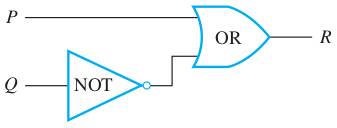
\includegraphics[scale=0.5]{../images/2.4.1.png}
\end{figure}
input signals: $P = 1$ and $Q = 1$

\begin{proof}
$R = 1$
\end{proof}

\subsection{Exercise 2}
\begin{figure}[ht!]
\centering
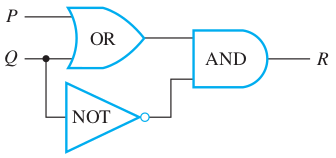
\includegraphics[scale=0.5]{../images/2.4.2.png}
\end{figure}
input signals: $P = 1$ and $Q = 0$

\begin{proof}
$R = 1$
\end{proof}

\subsection{Exercise 3}
\begin{figure}[ht!]
\centering
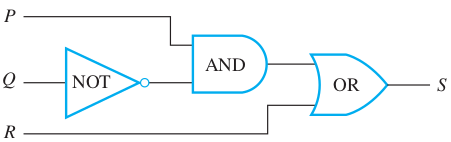
\includegraphics[scale=0.5]{../images/2.4.3.png}
\end{figure}
input signals: $P = 1, Q = 0, R = 0$

\begin{proof}
$S = 1$
\end{proof}

\subsection{Exercise 4}
\begin{figure}[ht!]
\centering
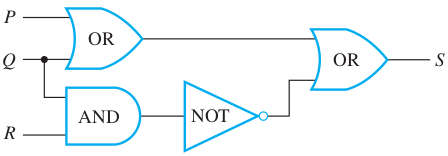
\includegraphics[scale=0.5]{../images/2.4.4.png}
\end{figure}
input signals: $P = 0, Q = 0, R = 0$

\begin{proof}
$S = 1$
\end{proof}

{\bf \color{cyan} In $5-8$, write an input/output table for the circuit in the referenced exercise.}

\subsection{Exercise 5}
Exercise 1

\begin{proof}
$$
\begin{array}{|cc|c|}
\hline
P&Q&R\\
\hline
1&1&1\\
\hline
1&0&0\\
\hline
0&1&1\\
\hline
0&0&0\\
\hline
\end{array}
$$
\end{proof}

\subsection{Exercise 6}
Exercise 2

\begin{proof}
$$
\begin{array}{|cc|c|}
\hline
P&Q&R\\
\hline
1&1&0\\
\hline
1&0&1\\
\hline
0&1&0\\
\hline
0&0&0\\
\hline
\end{array}
$$
\end{proof}

\subsection{Exercise 7}
Exercise 3

\begin{proof}
$$
\begin{array}{|ccc|c|}
\hline
P&Q&R&S\\
\hline
1&1&1&0\\
\hline
1&1&0&1\\
\hline
1&0&1&0\\
\hline
1&0&0&0\\
\hline
0&1&1&1\\
\hline
0&1&0&1\\
\hline
0&0&1&0\\
\hline
0&0&0&0\\
\hline
\end{array}
$$
\end{proof}

\subsection{Exercise 8}
Exercise 4

\begin{proof}
$$
\begin{array}{|ccc|c|}
\hline
P&Q&R&S\\
\hline
1&1&1&1\\
\hline
1&1&0&1\\
\hline
1&0&1&1\\
\hline
1&0&0&1\\
\hline
0&1&1&1\\
\hline
0&1&0&1\\
\hline
0&0&1&1\\
\hline
0&0&0&1\\
\hline
\end{array}
$$
\end{proof}

{\bf \color{cyan} In $9-12$, find the Boolean expression that corresponds to the circuit in the referenced exercise.}

\subsection{Exercise 9}
Exercise 1

\begin{proof}
$P \vee {\sim Q}$
\end{proof}

\subsection{Exercise 10}
Exercise 2

\begin{proof}
$(P \vee Q) \wedge {\sim Q}$
\end{proof}

\subsection{Exercise 11}
Exercise 3

\begin{proof}
$(P \wedge {\sim Q}) \vee R$
\end{proof}

\subsection{Exercise 12}
Exercise 4

\begin{proof}
$(P \vee Q) \vee {\sim (Q \wedge R)}$
\end{proof}

{\bf \color{cyan} Construct circuits for the Boolean expressions in $13-17$.}

\subsection{Exercise 13}
${\sim P} \vee Q$

\begin{proof}
\begin{figure}[ht!]
\centering
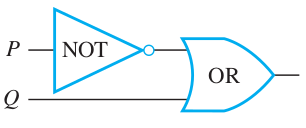
\includegraphics[scale=0.5]{../images/2.4.13.png}
\end{figure}
\end{proof}

\subsection{Exercise 14}
${\sim(P \vee Q)}$

\begin{proof}
\begin{figure}[ht!]
\centering
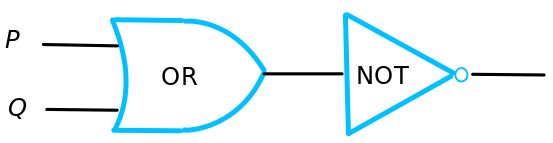
\includegraphics[scale=0.3]{../images/2.4.14.png}
\end{figure}
\end{proof}

\subsection{Exercise 15}
$P \vee ({\sim P} \wedge {\sim Q})$

\begin{proof}
\begin{figure}[ht!]
\centering
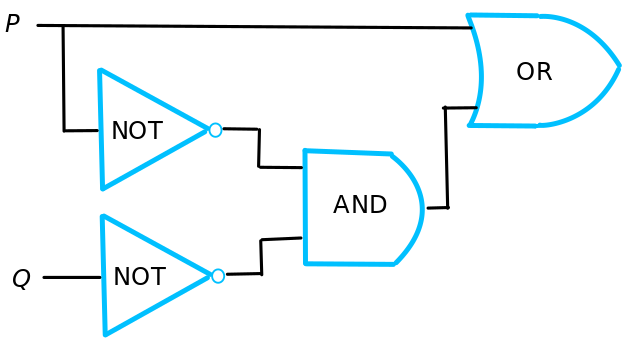
\includegraphics[scale=0.3]{../images/2.4.15.png}
\end{figure}
\end{proof}

\subsection{Exercise 16}
$(P \wedge Q) \vee {\sim R}$

\begin{proof}
\begin{figure}[ht!]
\centering
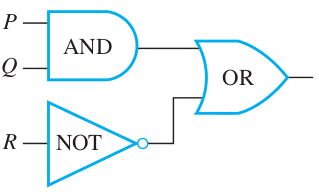
\includegraphics[scale=0.5]{../images/2.4.16.png}
\end{figure}
\end{proof}

\subsection{Exercise 17}
$(P \wedge {\sim Q}) \vee ({\sim P} \wedge R)$

\begin{proof}
\begin{figure}[ht!]
\centering
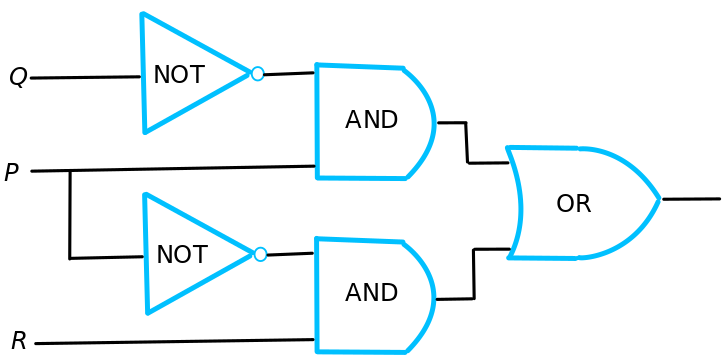
\includegraphics[scale=0.3]{../images/2.4.17.png}
\end{figure}
\end{proof}

{\bf \color{cyan} For each of the tables in 18–21, construct (a) a Boolean expression having the given table as its truth table and (b) a circuit having the given table as its input/output table.}

\subsection{Exercise 18}
$$
\begin{array}{|ccc|c|}
\hline
P&Q&R&S\\
\hline
1&1&1&0\\
\hline
1&1&0&1\\
\hline
1&0&1&0\\
\hline
1&0&0&0\\
\hline
0&1&1&1\\
\hline
0&1&0&0\\
\hline
0&0&1&0\\
\hline
0&0&0&0\\
\hline
\end{array}
$$

\begin{proof}
$(P \wedge Q \wedge {\sim R}) \vee ({\sim P} \wedge Q \wedge R)$

\begin{figure}[ht!]
\centering
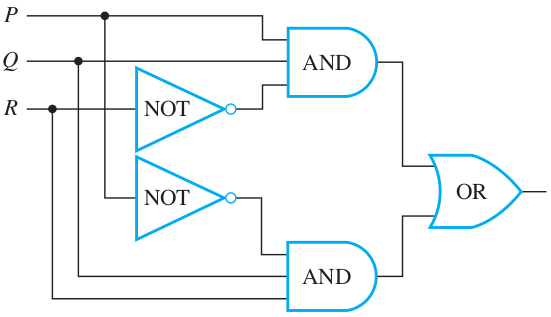
\includegraphics[scale=0.5]{../images/2.4.18.png}
\end{figure}
\end{proof}

\subsection{Exercise 19}
$$
\begin{array}{|ccc|c|}
\hline
P&Q&R&S\\
\hline
1&1&1&0\\
\hline
1&1&0&1\\
\hline
1&0&1&0\\
\hline
1&0&0&1\\
\hline
0&1&1&0\\
\hline
0&1&0&1\\
\hline
0&0&1&0\\
\hline
0&0&0&0\\
\hline
\end{array}
$$

\begin{proof}
$(P \wedge Q \wedge {\sim R}) \vee (P \wedge {\sim Q} \wedge {\sim R}) \vee ({\sim P} \wedge Q \wedge {\sim R})$

\begin{figure}[ht!]
\centering
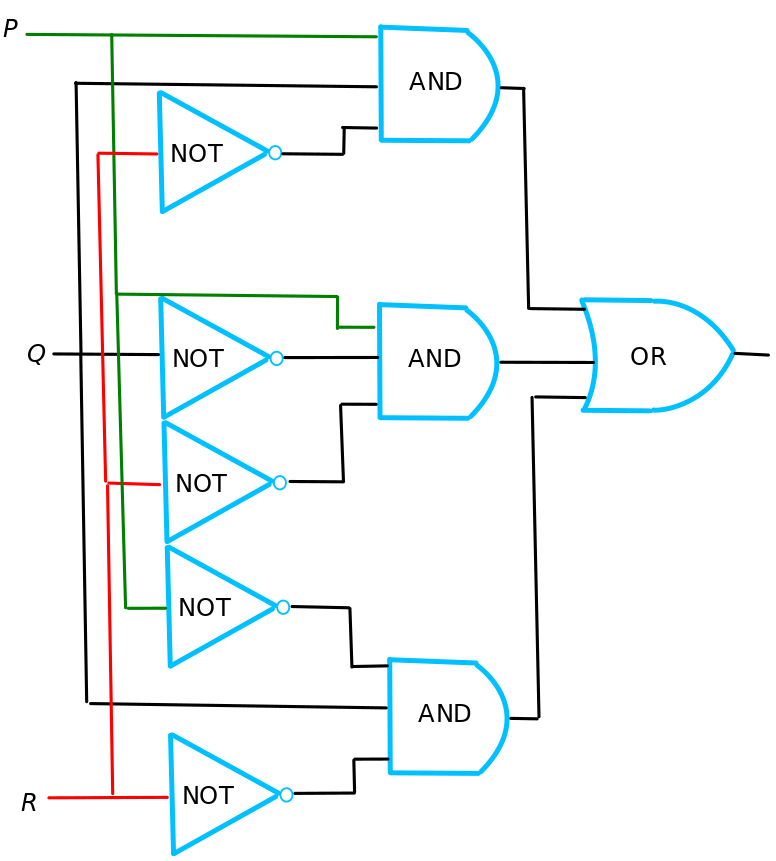
\includegraphics[scale=0.3]{../images/2.4.19.png}
\end{figure}
\end{proof}

\subsection{Exercise 20}
$$
\begin{array}{|ccc|c|}
\hline
P&Q&R&S\\
\hline
1&1&1&1\\
\hline
1&1&0&0\\
\hline
1&0&1&1\\
\hline
1&0&0&0\\
\hline
0&1&1&0\\
\hline
0&1&0&0\\
\hline
0&0&1&0\\
\hline
0&0&0&1\\
\hline
\end{array}
$$

\begin{proof}
$(P \wedge Q \wedge R) \vee (P \wedge {\sim Q} \wedge R) \vee ({\sim P} \wedge {\sim Q} \wedge {\sim R})$

\begin{figure}[ht!]
\centering
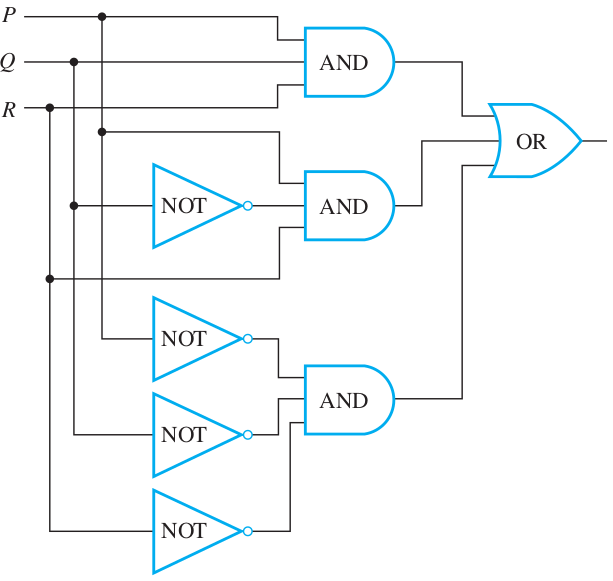
\includegraphics[scale=0.4]{../images/2.4.20.png}
\end{figure}
\end{proof}

\subsection{Exercise 21}
$$
\begin{array}{|ccc|c|}
\hline
P&Q&R&S\\
\hline
1&1&1&0\\
\hline
1&1&0&1\\
\hline
1&0&1&0\\
\hline
1&0&0&0\\
\hline
0&1&1&1\\
\hline
0&1&0&1\\
\hline
0&0&1&0\\
\hline
0&0&0&0\\
\hline
\end{array}
$$

\begin{proof}
$(P \wedge Q \wedge {\sim R}) \vee ({\sim P} \wedge Q \wedge R) \vee ({\sim P} \wedge Q \wedge {\sim R})$

\begin{figure}[ht!]
\centering
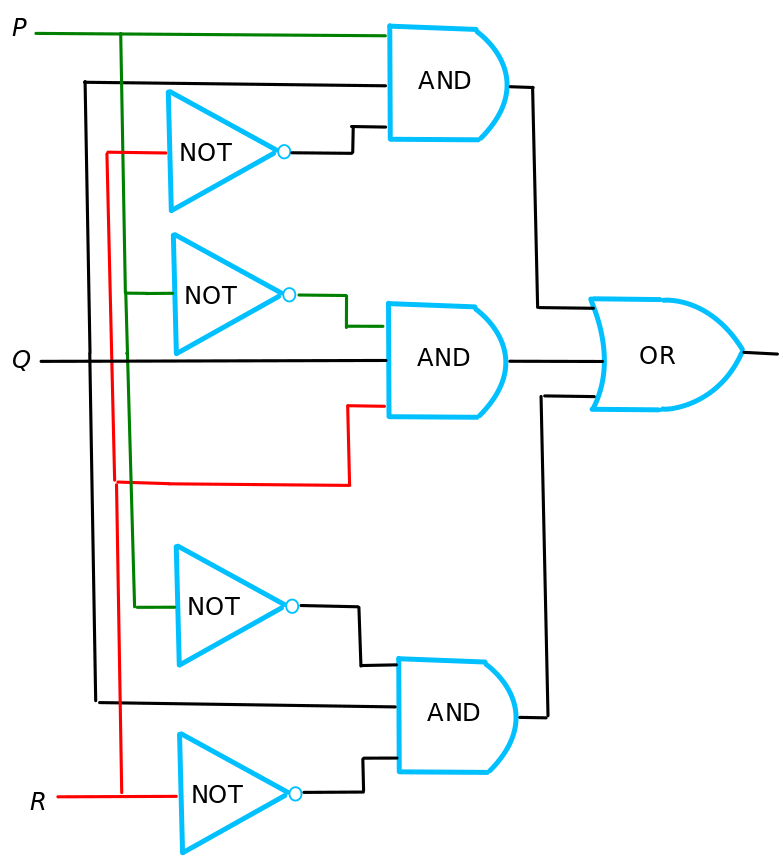
\includegraphics[scale=0.3]{../images/2.4.21.png}
\end{figure}
\end{proof}

\subsection{Exercise 22}
Design a circuit to take input signals $P, Q$, and $R$ and output a 1 if, and only if, $P$ and $Q$ have the same value and $Q$ and $R$ have opposite values.

\begin{proof}
The input/output table is:

$$
\begin{array}{|ccc|c|}
\hline
& \color{cyan}\text{Input} & & \color{cyan}\text{Output} \\
\hline
P&Q&R&S\\
\hline
1&1&1&0\\
\hline
1&1&0&1\\
\hline
1&0&1&0\\
\hline
1&0&0&0\\
\hline
0&1&1&0\\
\hline
0&1&0&0\\
\hline
0&0&1&1\\
\hline
0&0&0&0\\
\hline
\end{array}
$$

A formula is: $(P \wedge Q \wedge {\sim R}) \vee ({\sim P} \wedge {\sim Q} \wedge R)$.

One circuit (among many) having this input/output table is the following:

\begin{figure}[ht!]
\centering
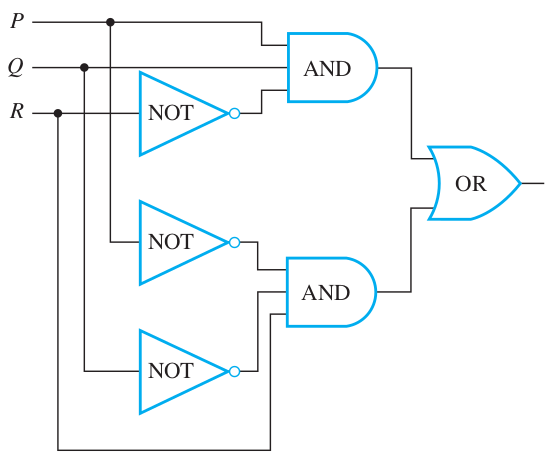
\includegraphics[scale=0.5]{../images/2.4.22.png}
\end{figure}
\end{proof}

\subsection{Exercise 23}
Design a circuit to take input signals $P, Q$, and $R$ and output a 1 if, and only if, all three of $P, Q$, and $R$ have the same value.

\begin{proof}
The input/output table is:

$$
\begin{array}{|ccc|c|}
\hline
& \color{cyan}\text{Input} & & \color{cyan}\text{Output} \\
\hline
P&Q&R&S\\
\hline
1&1&1&1\\
\hline
1&1&0&0\\
\hline
1&0&1&0\\
\hline
1&0&0&0\\
\hline
0&1&1&0\\
\hline
0&1&0&0\\
\hline
0&0&1&0\\
\hline
0&0&0&1\\
\hline
\end{array}
$$

A formula (among many) is: $(P \wedge Q \wedge R) \vee ({\sim P} \wedge {\sim Q} \wedge {\sim R})$.

One circuit (among many) having this input/output table is the following:

\begin{figure}[ht!]
\centering
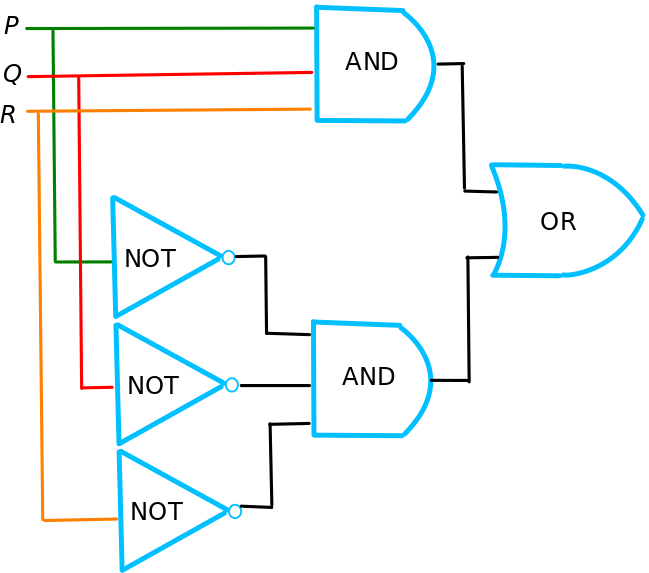
\includegraphics[scale=0.3]{../images/2.4.23.png}
\end{figure}
\end{proof}

\subsection{Exercise 24}
The lights in a classroom are controlled by two switches: one at the back of the room and one at the front. Moving either switch to the opposite position turns the lights off if they are on and on if they are off. Assume the lights have been installed so that when both switches are in the down position, the lights are off. Design a circuit to control the switches.

\begin{proof}
Let $P$ and $Q$ represent the positions of the switches in the classroom, with 0 being “down” and 1 being “up.” Let $R$ represent the condition of the light, with 0 being “off” and 1 being “on.” Initially, $P = Q = 0$ and $R = 0$. If either $P$ or $Q$ (but not both) is changed to 1, the light turns on. So when $P = 1$ and $Q = 0$, then $R = 1$, and when $P = 0$ and $Q = 1$, then $R = 1$. Thus when one switch is up and the other is down the light is on, and hence moving the switch that is down to the up position turns the light off. So when $P = 1$ and $Q = 1$, then $R = 0$. It follows that the input/output table has the following appearance:

$$
\begin{array}{|cc|c|}
\hline
\text{input} & \text{input} & \text{output} \\
\hline
P&Q&R\\
\hline
1&1&0\\
\hline
1&0&1\\
\hline
0&1&1\\
\hline
0&0&0\\
\hline
\end{array}
$$

One circuit (among many) having this input/output table is the following:

\begin{figure}[ht!]
\centering
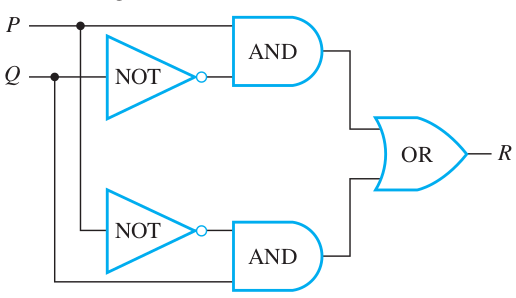
\includegraphics[scale=0.5]{../images/2.4.24.png}
\end{figure}
\end{proof}

\subsection{Exercise 25}
An alarm system has three different control panels in three different locations. To enable the system, switches in at least two of the panels must be in the on position. If fewer than two are in the on position, the system is disabled. Design a circuit to control the switches.

\begin{proof}
Let $P, Q, R$ represent the switches in the 3 control panels. Let $S$ represent the overall system. It follows that the input/output table has the following appearance:

$$
\begin{array}{|ccc|c|}
\hline
& \color{cyan}\text{Input} & & \color{cyan}\text{Output} \\
\hline
P&Q&R&S\\
\hline
1&1&1&1\\
\hline
1&1&0&1\\
\hline
1&0&1&1\\
\hline
1&0&0&0\\
\hline
0&1&1&1\\
\hline
0&1&0&0\\
\hline
0&0&1&0\\
\hline
0&0&0&0\\
\hline
\end{array}
$$

A formula (among many) is:
$$
(P \wedge Q \wedge R) \vee (P \wedge Q \wedge {\sim R}) \vee (P \wedge {\sim Q} \wedge R) \vee ({\sim P} \wedge Q \wedge R)
$$
In this form, the circuit would be too complicated. Let's simplify.

By the distributive law, the negation law and the identity law, we can simplify the first two terms as:
$$
(P \wedge Q \wedge R) \vee (P \wedge Q \wedge {\sim R}) \equiv (P \wedge Q) \wedge (R \vee {\sim R}) \equiv (P \wedge Q) \wedge \true \equiv P \wedge Q
$$
By the distributive law we can simplify the last two terms as:
$$
(P \wedge {\sim Q} \wedge R) \vee ({\sim P} \wedge Q \wedge R) \equiv R \wedge ((P \wedge {\sim Q}) \vee ({\sim P} \wedge Q))
$$
If you allow me to cheat a little bit, the portion $((P \wedge {\sim Q}) \vee ({\sim P} \wedge Q))$ is equivalent to the exclusive or of $P$ and $Q$, namely $P \oplus Q$.

So the overall formula simplifies to: $(P \wedge Q) \vee (R \wedge (P \oplus Q))$.

One circuit (among many) having this input/output table is the following:

\begin{figure}[ht!]
\centering
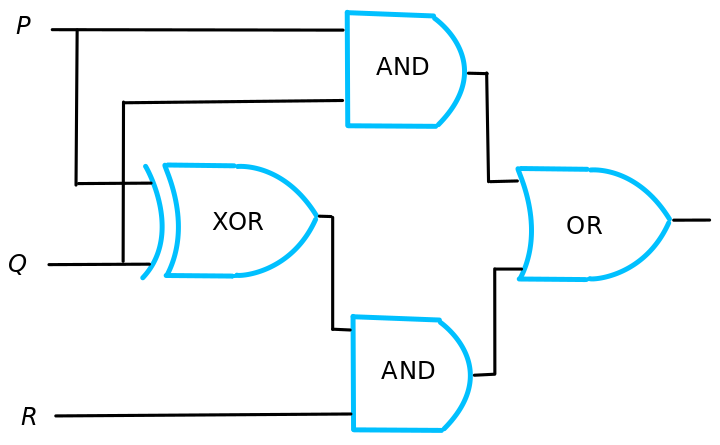
\includegraphics[scale=0.3]{../images/2.4.25.png}
\end{figure}
\end{proof}

{\bf \color{cyan} Use the properties listed in Theorem 2.1.1 to show that each pair of circuits in $26-29$ have the same input/output table. (Find the Boolean expressions for the circuits and
show that they are logically equivalent when regarded as statement forms.)}

\subsection{Exercise 26}
\begin{figure}[ht!]
\centering
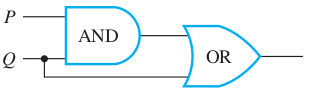
\includegraphics[scale=0.5]{../images/2.4.26.a.png}
\end{figure}

\begin{figure}[ht!]
\centering
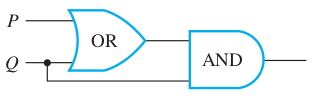
\includegraphics[scale=0.5]{../images/2.4.26.b.png}
\end{figure}

\begin{proof}
The Boolean expression for the first is $(P \wedge Q) \vee Q$ and for the second it is $(P \vee Q) \wedge Q$. We must show that if these expressions are regarded as statement forms, then they are logically equivalent. Now
$$
\begin{array}{rcll}
(P \wedge Q) \vee Q & \equiv & Q \vee (P \wedge Q) & \text{\color{cyan}by the commutative law} \\
& \equiv & (Q \vee P) \wedge (Q \vee Q) & \text{\color{cyan}by the distributive law} \\
& \equiv & (Q \vee P) \wedge Q & \text{\color{cyan}by the idempotent law} \\
& \equiv & (P \vee Q) \wedge Q & \text{\color{cyan}by the commutative law} \\
\end{array}
$$
Alternatively, by the absorption laws, both statement forms are logically equivalent to $Q$.
\end{proof}

\subsection{Exercise 27}
\begin{figure}[ht!]
\centering
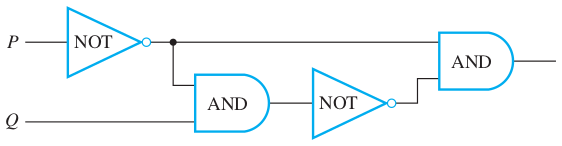
\includegraphics[scale=0.5]{../images/2.4.27.a.png}
\end{figure}

\begin{figure}[ht!]
\centering
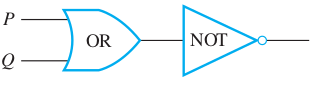
\includegraphics[scale=0.5]{../images/2.4.27.b.png}
\end{figure}

\begin{proof}
The first is ${\sim P} \wedge {\sim ({\sim P} \wedge Q)}$ and the second is ${\sim (P \vee Q)}$. 

If we apply De Morgan laws to both, we get: ${\sim P} \wedge (P \vee {\sim Q})$ and ${\sim P} \wedge {\sim Q}$. 

If we apply the distributive law, the negation law and the identity law to the first, we get: 

${\sim P} \wedge (P \vee {\sim Q}) \equiv ({\sim P} \wedge P) \vee ({\sim P} \wedge {\sim Q}) \equiv \false \vee ({\sim P} \wedge {\sim Q}) \equiv {\sim P} \wedge {\sim Q}$.

So they are both equivalent to ${\sim P} \wedge {\sim Q}$.
\end{proof}

\subsection{Exercise 28}
\begin{figure}[ht!]
\centering
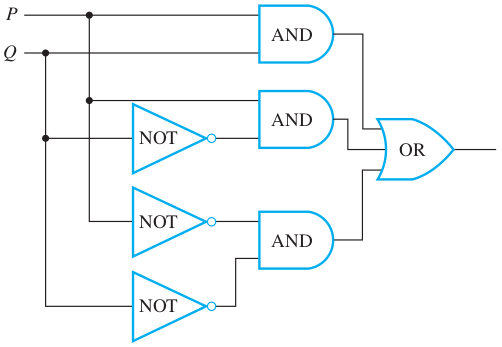
\includegraphics[scale=0.5]{../images/2.4.28.a.png}
\end{figure}

\begin{figure}[ht!]
\centering
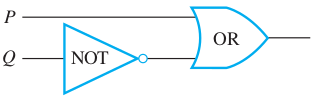
\includegraphics[scale=0.5]{../images/2.4.28.b.png}
\end{figure}

\begin{proof}
First is $(P \wedge Q) \vee (P \wedge {\sim Q}) \vee ({\sim P} \wedge {\sim Q})$ and second is $P \vee {\sim Q}$.

$(P \wedge Q) \vee (P \wedge {\sim Q}) \vee ({\sim P} \wedge {\sim Q})$
$$
\begin{array}{cll}
\equiv & (P \wedge (Q \vee {\sim Q})) \vee ({\sim P} \wedge {\sim Q}) & \text{\color{cyan}by distributive law} \\
\equiv & (P \wedge \true) \vee ({\sim P} \wedge {\sim Q}) & \text{\color{cyan}by negation law} \\
\equiv & P \vee ({\sim P} \wedge {\sim Q}) & \text{\color{cyan}by identity law} \\
\equiv & (P \vee {\sim P}) \wedge (P \vee {\sim Q}) & \text{\color{cyan}by distributive law} \\
\equiv & \true \wedge (P \vee {\sim Q}) & \text{\color{cyan}by negation law} \\
\equiv & P \vee {\sim Q} & \text{\color{cyan}by identity law} \\
\end{array}
$$
So they are logically equivalent.
\end{proof}

\subsection{Exercise 29}
\begin{figure}[ht!]
\centering
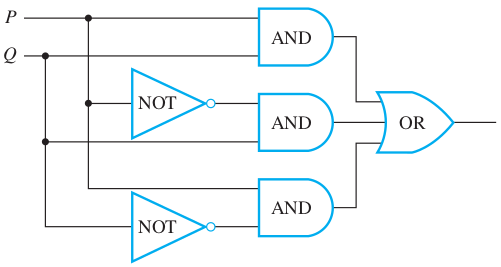
\includegraphics[scale=0.5]{../images/2.4.29.a.png}
\end{figure}

\begin{figure}[ht!]
\centering
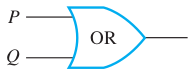
\includegraphics[scale=0.5]{../images/2.4.29.b.png}
\end{figure}

\begin{proof}
First is $(P \wedge Q) \vee ({\sim P} \wedge Q) \vee (P \wedge {\sim Q})$ and second is $P \vee Q$.

$(P \wedge Q) \vee ({\sim P} \wedge Q) \vee (P \wedge {\sim Q})$
$$
\begin{array}{cll}
\equiv & ((P \vee {\sim P}) \wedge Q) \vee (P \wedge {\sim Q}) & \text{\color{cyan}by distributive law} \\
\equiv & (\true \wedge Q) \vee (P \wedge {\sim Q}) & \text{\color{cyan}by negation law} \\
\equiv & Q \vee (P \wedge {\sim Q}) & \text{\color{cyan}by identity law} \\
\equiv & (Q \vee P) \wedge (Q \vee {\sim Q}) & \text{\color{cyan}by distributive law} \\
\equiv & (Q \vee P) \wedge \true & \text{\color{cyan}by negation law} \\
\equiv & Q \vee P & \text{\color{cyan}by identity law} \\
\equiv & P \vee Q & \text{\color{cyan}by commutative law} \\
\end{array}
$$
So they are logically equivalent.
\end{proof}

{\bf \color{cyan} For the circuits corresponding to the Boolean expressions in each of 30 and 31 there is an equivalent circuit with at most two logic gates. Find such a circuit.}

\subsection{Exercise 30}
$(P \wedge Q) \vee ({\sim P} \wedge Q) \vee ({\sim P} \wedge {\sim Q})$

\begin{proof}
$(P \wedge Q) \vee ({\sim P} \wedge Q) \vee ({\sim P} \wedge {\sim Q})$
$$
\begin{array}{cll}
\equiv & (P \wedge Q) \vee (({\sim P} \wedge Q) \vee ({\sim P} \wedge {\sim Q})) & \text{\color{cyan}by associativity} \\
\equiv & (P \wedge Q) \vee ({\sim P} \wedge (Q \vee {\sim Q})) & \text{\color{cyan}by the distributive law} \\
\equiv & (P \wedge Q) \vee ({\sim P} \wedge \true) & \text{\color{cyan}by the negation law} \\
\equiv & (P \wedge Q) \vee {\sim P} & \text{\color{cyan}by the identity law} \\
\equiv & ({\sim P} \vee P) \wedge ({\sim P} \vee Q) & \text{\color{cyan}by the distributive law} \\
\equiv & \true \wedge ({\sim P} \vee Q) & \text{\color{cyan}by the negation law} \\
\equiv & {\sim P} \vee Q & \text{\color{cyan}by the identity law} \\
\end{array}
$$
The following is, therefore, a circuit with at most two logic gates that has the same input/output table as the circuit corresponding to the given expression.
\begin{figure}[ht!]
\centering
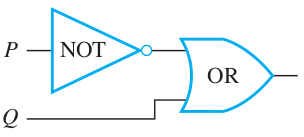
\includegraphics[scale=0.5]{../images/2.4.30.png}
\end{figure}
\end{proof}

\subsection{Exercise 31}
$({\sim P} \wedge {\sim Q}) \vee ({\sim P} \wedge Q) \vee (P \wedge {\sim Q})$

\begin{proof}
$({\sim P} \wedge {\sim Q}) \vee ({\sim P} \wedge Q) \vee (P \wedge {\sim Q})$
$$
\begin{array}{cll}
\equiv & ({\sim P} \wedge ({\sim Q} \vee Q)) \vee (P \wedge {\sim Q}) & \text{\color{cyan}by the distributive law} \\
\equiv & ({\sim P} \wedge \true) \vee (P \wedge {\sim Q}) & \text{\color{cyan}by the negation law} \\
\equiv & {\sim P} \vee (P \wedge {\sim Q}) & \text{\color{cyan}by the identity law} \\
\equiv & ({\sim P} \vee P) \wedge ({\sim P} \vee {\sim Q}) & \text{\color{cyan}by the distributive law} \\
\equiv & \true \wedge ({\sim P} \vee {\sim Q}) & \text{\color{cyan}by the negation law} \\
\equiv & {\sim P} \vee {\sim Q} & \text{\color{cyan}by the identity law} \\
\equiv & {\sim (P \wedge Q)} & \text{\color{cyan}by De Morgan's law} \\
\end{array}
$$
The following is, therefore, a circuit with at most two logic gates that has the same input/output table as the circuit corresponding to the given expression.
\begin{figure}[ht!]
\centering
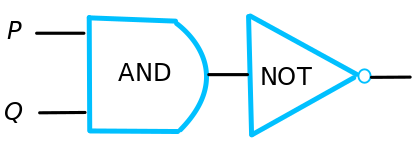
\includegraphics[scale=0.4]{../images/2.4.31.png}
\end{figure}
\end{proof}

\subsection{Exercise 32}
The Boolean expression for the circuit in Example 2.4.5 is
$$
(P \wedge Q \wedge R) \vee (P \wedge {\sim Q} \wedge R) \vee (P \wedge {\sim Q}\wedge {\sim R})
$$
(a disjunctive normal form). Find a circuit with at most three logic gates that is equivalent to this circuit.

\begin{proof}
$(P \wedge Q \wedge R) \vee (P \wedge {\sim Q} \wedge R) \vee (P \wedge {\sim Q}\wedge {\sim R})$
$$
\begin{array}{cll}
\equiv & [(P \wedge R) \wedge (Q \vee {\sim Q})] \vee (P \wedge {\sim Q}\wedge {\sim R}) & \text{\color{cyan}by distributive law} \\
\equiv & [(P \wedge R) \wedge \true] \vee (P \wedge {\sim Q}\wedge {\sim R}) & \text{\color{cyan}by negation law} \\
\equiv & (P \wedge R) \vee (P \wedge {\sim Q}\wedge {\sim R}) & \text{\color{cyan}by identity law} \\
\equiv & P \wedge (R \vee ({\sim Q} \wedge {\sim R})) & \text{\color{cyan}by distributive law} \\
\equiv & P \wedge (R \vee {\sim Q}) \wedge (R \vee {\sim R})) & \text{\color{cyan}by distributive law} \\
\equiv & P \wedge ((R \vee {\sim Q}) \wedge \true) & \text{\color{cyan}by negation law} \\
\equiv & P \wedge (R \vee {\sim Q}) & \text{\color{cyan}by identity law} \\
\end{array}
$$
\begin{figure}[ht!]
\centering
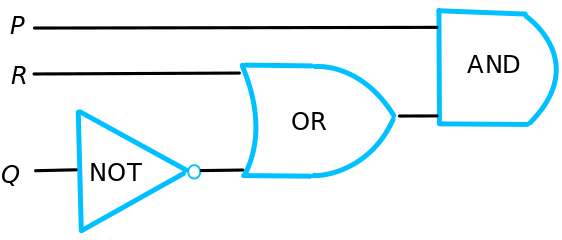
\includegraphics[scale=0.3]{../images/2.4.32.png}
\end{figure}
\end{proof}

\subsection{Exercise 33}
\subsubsection{(a)}
Show that for the Sheffer stroke $|$,
$$
P \wedge Q \equiv (P | Q) | (P | Q)
$$

\begin{proof}
$(P | Q) | (P | Q)$
$$
\begin{array}{cll}
\equiv & {\sim (P \wedge Q)} | {\sim (P \wedge Q)} & \text{\color{cyan}by definition of Sheffer stroke} \\
\equiv & {\sim ({\sim (P \wedge Q)} \wedge {\sim (P \wedge Q)})} & \text{\color{cyan}by definition of Sheffer stroke} \\
\equiv & (P \wedge Q) \vee (P \wedge Q) & \text{\color{cyan}by De Morgan laws} \\
\equiv & P \wedge Q & \text{\color{cyan}by idempotent law} \\
\end{array}
$$
\end{proof}

\subsubsection{(b)}
Use the results of Example 2.4.7 and part (a) above to write $P \wedge ({\sim Q} \vee R)$ using only Sheffer strokes.

\begin{proof}
${\sim Q} \vee R$ is logically equivalent to ${\sim (Q \wedge {\sim R})}$, which is $Q | {\sim R}$ by definition of Sheffer stroke. 

By Example 2.4.7 ${\sim R} \equiv R | R$, so ${\sim Q} \vee R \equiv Q | (R | R)$.

By part (a) above $P \wedge ({\sim Q} \vee R) \equiv (P|({\sim Q} \vee R)) | (P|({\sim Q} \vee R))$.

Using the two pieces above, we get $P \wedge ({\sim Q} \vee R) \equiv (P|(Q | (R | R))) | (P|(Q | (R | R)))$.
\end{proof}

\subsection{Exercise 34}
Show that the following logical equivalences hold for the Peirce arrow $\downarrow$, where $P \downarrow Q \equiv {\sim (P \vee Q)}$.

\subsubsection{(a)}
${\sim P} \equiv P \downarrow P$

\begin{proof}
$P \downarrow P$
$$
\begin{array}{cll}
\equiv & {\sim(P \vee P)} & \text{\color{cyan}by definition of Peirce arrow} \\
\equiv & {\sim P} \wedge {\sim P} & \text{\color{cyan}by De Morgan laws} \\
\equiv & {\sim P} & \text{\color{cyan}by idempotent law} \\
\end{array}
$$
\end{proof}

\subsubsection{(b)}
$P \vee Q \equiv (P \downarrow Q) \downarrow (P \downarrow Q)$

\begin{proof}
$$
\begin{array}{rcll}
(P \downarrow Q) \downarrow (P \downarrow Q) & \equiv & {\sim (P \downarrow Q)} & \text{\color{cyan}by part (a)} \\
 & \equiv & {\sim[{\sim (P \vee Q)}]} & \text{\color{cyan}by definition of } \downarrow \\
 & \equiv & P \vee Q& \text{\color{cyan}by the double negation law} \\
\end{array}
$$
\end{proof}

\subsubsection{(c)}
$P \wedge Q \equiv (P \downarrow P) \downarrow (Q \downarrow Q)$

\begin{proof}
$(P \downarrow P) \downarrow (Q \downarrow Q)$
$$
\begin{array}{cll}
\equiv & {\sim P} \downarrow {\sim Q} & \text{\color{cyan}by part (a)} \\
\equiv & {\sim ({\sim P} \vee {\sim Q})} & \text{\color{cyan}by definition of Peirce arrow} \\
\equiv & {\sim {\sim P}} \wedge {\sim {\sim Q}} & \text{\color{cyan}by De Morgan laws} \\
\equiv & P \wedge Q & \text{\color{cyan}by double negation laws} \\
\end{array}
$$
\end{proof}

\subsubsection{(d)}
Write $P \to Q$ using Peirce arrows only.

Hint: Use the results of exercise 13 of Section 2.2 and part (a) and (c) of this exercise.

\begin{proof}
$P \to Q$
$$
\begin{array}{cll}
\equiv & {\sim P} \vee Q & \text{\color{cyan}by Exercise 2.2.13} \\
\equiv & (P \downarrow P) \vee Q & \text{\color{cyan}by part (a)} \\
\equiv & ((P \downarrow P) \downarrow Q) \downarrow ((P \downarrow P) \downarrow Q) & \text{\color{cyan}by part (b)} \\
\end{array}
$$
\end{proof}

\subsubsection{(e)}
Write $P \bic Q$ using Peirce arrows only.

\begin{proof}
$P \bic Q$
$$
\begin{array}{cll}
\equiv & (P \to Q) \wedge (Q \to P) & \text{\color{cyan}by def of } \bic \\
\equiv & [((P \downarrow P) \downarrow Q) \downarrow ((P \downarrow P) \downarrow Q)] \wedge [((Q \downarrow Q) \downarrow P) \downarrow ((Q \downarrow Q) \downarrow P)] & \text{\color{cyan}by part (d)} \\
\equiv & ([((P \downarrow P) \downarrow Q) \downarrow ((P \downarrow P) \downarrow Q)] \downarrow [((P \downarrow P) \downarrow Q) \downarrow ((P \downarrow P) \downarrow Q)])\\ 
& ([((Q \downarrow Q) \downarrow P) \downarrow ((Q \downarrow Q) \downarrow P)] \downarrow [((Q \downarrow Q) \downarrow P) \downarrow ((Q \downarrow Q) \downarrow P)]) & \text{\color{cyan}by part (c)} \\
\end{array}
$$
\end{proof}

\end{document}
